\documentclass[
%%%%% Styles and Sizes
%10pt,
%11pt,
%12pt,
fancyheadings, % headings with seplines and logo
%
%%%%% Printing, Color and Binding
%a4paper, 
%a5paper,
%twoside, % single sided printout
%oneside, % duplex printout (default)
%% binding correction is used to compensate for the paper lost during binding
%% of the document
%BCOR=0.7cm, % binding correction
%nobcorignoretitle, % do not ignore BCOR for title page
%% the following two options only concern the graphics included by the document
%% class
%grayscaletitle, % keep the title in grayscale
%grayscalebody, % keep the rest of the document in grayscale
%
%%%%% expert options: your mileage may vary
%baseclass=..., % special option to use a different document baseclass
]{stsreprt}

% Information for the Titlepage
\author{Lennart Mühlhahn}
\title{Mutation-Based Accuracy Improvements in Neural Networks using Spectrum-Based Fault Localization}
\date{\today}
\subject{Bachelor Thesis}
\professor{Prof. Dr. Sibylle Schupp}
\advisor{Daniel Rashedi}

\usepackage[utf8]{inputenc}

% Font and Fontencoding Magic
% FAQ: 
% http://tex.stackexchange.com/questions/664/why-should-i-use-usepackaget1fontenc
% http://en.wikipedia.org/wiki/Computer_Modern
% http://tex.stackexchange.com/questions/1390/latin-modern-vs-cm-super
\usepackage[T1]{fontenc}
\usepackage{lmodern}
%\usepackage{fix-cm}

% to include bibliography
\usepackage{biblatex}
\addbibresource{Bachelorarbeit.bib}
\usepackage[breaklinks=true,hidelinks]{hyperref}
\usepackage{amsmath}
\usepackage{amsfonts}
\usepackage{pgfplots}
\usepackage{tikz}
\usepackage{multirow}
\usepackage{listings}
\usepackage{lscape}
\usetikzlibrary{matrix, positioning, shapes.geometric, arrows}
\usepackage{xcolor}
\usepackage{listofitems} % for \readlist to create arrays
\tikzstyle{mynode}=[thick,draw=blue,fill=blue!20,circle,minimum size=22]
\pgfplotsset{compat=1.17}

\definecolor{codegreen}{rgb}{0,0.6,0}
\definecolor{codegray}{rgb}{0.5,0.5,0.5}
\definecolor{codepurple}{rgb}{0.58,0,0.82}
\definecolor{backcolour}{rgb}{0.95,0.95,0.92}

\lstdefinestyle{mystyle}{
    backgroundcolor=\color{backcolour},
    commentstyle=\color{codegreen},
    keywordstyle=\color{magenta},
    numberstyle=\tiny\color{codegray},
    stringstyle=\color{codepurple},
    basicstyle=\ttfamily\footnotesize,
    breakatwhitespace=false,
    breaklines=true,
    captionpos=b,
    keepspaces=true,
    numbers=left,
    numbersep=5pt,
    showspaces=false,
    showstringspaces=false,
    showtabs=false,
    tabsize=2
}
\tikzstyle{startstop} = [rectangle, rounded corners,
minimum width=3cm,
minimum height=1cm,
text centered,
draw=black,
fill=red!30]

\tikzstyle{process} = [rectangle,
minimum width=3cm,
minimum height=1cm,
text centered,
text width=3cm,
draw=black,
fill=orange!30]

\tikzstyle{decision} = [diamond,
minimum width=2.5cm,
minimum height=2cm,
text width=1.5cm,
text centered,
draw=black,
fill=green!30]
\tikzstyle{arrow} = [thick,->,>=stealth]

\lstset{style=mystyle}
\usepackage{subcaption}

\begin{document}
\frontmatter
\maketitle
\chapter*{Declaration}
I, Lennart Mühlhahn, hereby affirm that the Bachelor's thesis titled “Mutation-Based Accuracy Improvements in Neural Networks using Spectrum-Based Fault Localization” is entirely my own work, completed independently and without unauthorized external help.

I have duly acknowledged and cited all instances of direct quotations and paraphrased content from other authors, ensuring that all such references are properly sourced.

\vspace{2cm} % Adjust vertical space as needed

\noindent
\begin{tabular}{@{}p{0.5\textwidth}p{0.5\textwidth}@{}}
    Hamburg, \today & \hfill \rule{6cm}{1pt} \\
    & \hfill Lennart Mühlhahn % Your name right-aligned
\end{tabular}
\chapter*{\centering \begin{normalsize}Abstract\end{normalsize}}
\begin{quotation}
    Abstract
\end{quotation}

\tableofcontents
\listoffigures{}
\lstlistoflistings
\mainmatter
\chapter{Introduction}\label{ch:introduction}
Deep Neural Networks (DNNs) \cite{lecun_deep_2015} are increasingly used in today's world and more capable than ever, and are often used in highly sensitive applications domains like medical diagnosis \cite{litjens_survey_2017} or autonomous vehicles \cite{bojarski_end_2016}.
DNNs are highly advanced in areas like image \cite{krizhevsky_imagenet_2012, ciresan_multi-column_2012}, video \cite{jiang_exploiting_2018}, or speech recognition \cite{hinton_deep_2012}.
There, the range of applications can range from simple recognition towards the end to end learning \cite{bojarski_end_2016}.

Especially because of the use of DNNs in safety-critical domains, it is from the uttermost urgency to ensure the safety of every user and every other person who is encountering these systems.
But how can we ensure the proper operation of the neural network, and find bad actors in neural networks and repair these neurons?

The Method we explored in this thesis is the mutation of neurons, which we first identified by using spectrum-based fault localization (SBFL).
While SBFL was already first successfully used in Eniser et al.'s DeepFault \cite{eniser_deepfault_2019} in conclusion with an input synthesizes guided by the suspiciousness values elicited by the SBFL, we want to go on to a more in-depth level and mutate the weights and biases based on these suspiciousness values.

For our approach, we first adapted the SBFL provided by DeepFault to today's versions of the TensorFlow framework, and the other used frameworks, afterwards we added the functions for the mutation of the weights and biases based on the ranked neuron locations provided by the SBFL\@.
The mutations either assign a value randomly, a predefined value, scales by a predefined or random value to the bias or weights of a neuron, we can also decapitate a neuron.
Then we added an algorithm to perform the mutation automatically by just providing the model, the data-set and the wished parameters.
We first perform the SBFL and rank the neuron in our network based on a suspiciousness measure, mutate the node, if wished, we train the model a further epoch.
Then we evaluate the model and if our break condition is met we give back the model, else we try to further improve the model by starting the loop with a new neuron again.

To evaluate our Approach, we used the Fashion-MNIST dataset by Xiao et al. \cite{xiao_fashion-mnist_2017}.
We used 4 model architectures, two Deep Neural Networks (DNN) and two Convolutional Neural Networks (CNN) to run our evaluation.
For the training, we haven't only used the full dataset to train the model, but also half and a quarter of the dataset.
Another thing that differentiated the models, we also trained them for either one or six epochs before using the algorithm.
We evaluated our approach based on the change of the performance (loss and accuracy) of the network against the baseline network.
If we further trained the model, we compared against the further trained reference model, else we compared the change against the initial performance of the model.

There by elicited an accuracy improvement in some cases up to in 25\% for the first three epochs of the algorithm for the not further trained models.
For the further trained models, we see an accuracy improvement of up to 7.5\%.
We see similar improvements in the loss values of the models.

Furthermore, we investigated the impact of the different suspiciousness measures and compared the usefulness against random choosing of the neurons.
Another thing we tried to elicit the effect of the different dataset sizes and the extent of the initial training.
Of course, we also tried to find the best configuration of the parameters for our Algorithm.
Exemplary of this is if the usage of an offset for the accuracy and loss, leads to better results.
For that, we also saw the need to evaluate the different break conditions for the algorithm.
And at last, we evaluated our different mutation functions and the assigned values.

To continue this Thesis, we will first give you some insights in to the techniques that are at the heart of our approach, neural networks, its testing and spectrum-based fault localization.
Then we give you a look at some other neural network repair methods and the first spectrum-based fault localization method for neural networks, DeepFault  \cite{eniser_deepfault_2019}.
Afterwards, we will provide a deep dive in to our approach until we present you our findings and an outlook to future research based on our work.
\chapter{Background}\label{ch:background}
In this chapter, we are going to present the background information that is necessary for our approach.
What are neural networks?
How can we test them, and what is spectrum-based fault localisation?
\section{Neural Networks}\label{sec:neural-networks}
Without further ado, we will discuss what neural networks are and how they are composed.
We describe what a layer is and what types there are.
For what do we need optimizers and activation functions and what types are there.
Neural Networks are useful in a multitude of fields like classification, regression, transcription, or machine translation \cite{goodfellow_deep_2016}.
Neuronal networks are composed of layers, which are composed of neurons.
The neuron is the computational component in a deep neural network.\\
A neuron transforms a vector of inputs $\mathbf{x}$ to the output $y$, $\mathbb{R}^n \to \mathbb{R}$
by using a vector of weights $\mathbf{w}$, a bias $b$ and an activation function $f$ as seen in equation \ref{eq: NeuralFunction}.
\begin{equation}
    y = f\left( \sum^n_{i=1} w_i\cdot x_i + b\right)
    \label{eq: NeuralFunction}
\end{equation}
For example the machine learning software library TensorFlow, which is based on Keras, uses by default Glorot uniform initializer \cite{noauthor_tfkeraslayersdense_2023,glorot_understanding_2010}, for the weights and initializes the bias with zeros.\\
Another important component, are the activation functions, one of the most common ones is the sigmoid function, which is today mostly used in output layers.
The rectified linear unit, short ReLU \cite{fukushima_cognitron_1975,glorot_deep_2011}, as seen in Function \ref{eq: relu}, enables a better training for a neural network compared to the formerly common sigmoid function.
\begin{equation}
    f(x) =
    \begin{cases}
        x& x > 0\\
        0& x <= 0
    \end{cases}
    \label{eq: relu}
\end{equation}
Another even more promising activation function is the Gaussian Error Linear Unit, short GELU, seen in function \ref{eq: relu}, which was proposed by Hendrycks and Gimpel in 2016 \cite{hendrycks_gaussian_2016} is used by natural language processing models like BERT \cite{devlin_bert_2019}.
It does not just set all negative values to zero like ReLU but weights them.
The differences can be seen in the figure. \ref{fig: activation function}
\begin{equation}
    f(x) = 0.5x\left ( 1+\tanh\left [ \sqrt{\frac{2}{\pi}}\left ( x+0.044715x^3 \right ) \right ] \right )
    \label{eq: gelu}
\end{equation}
\begin{figure}
    \centering
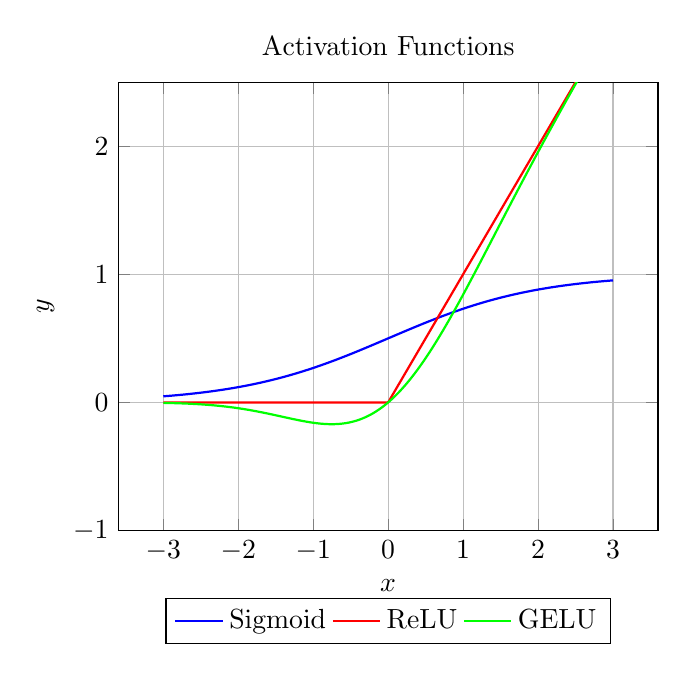
\begin{tikzpicture}
    \begin{axis}[
        title={Activation Functions},
        xlabel={$x$},
        ylabel={$y$},
        domain=-3:3, % Adjust the domain for a narrower x-axis range
        ymin=-1, % Set y-minimum
        ymax=2.5, % Set y-maximum
        samples=400, % Increase the number of samples for a smoother curve
        grid=both,
        legend style={at={(0.5,-0.15)}, anchor=north,legend columns=3},
      ]
      \addplot[blue, thick] {1/(1 + exp(-x))};
      \addplot[red, thick] {max(0, x)};
      \addplot[green, thick] {0.5*x*(1 + tanh(sqrt(2/pi)*(x + 0.044715*x^3)))};
      \legend{Sigmoid, ReLU, GELU}
    \end{axis}
  \end{tikzpicture}
  \caption{Activation Functions}
  \label{fig: activation function}
\end{figure}
The neurons are then combined into layers, in a Deep Neural Network (DNN) we have three types of Layers:
Input layers, output layers and the hidden layers.
There is one input and one output layer, but there is a plurality of hidden layers, as you can see in the figure \ref{fig: neural network}.
The input layer, processes the input for the hidden layers, for example, it converts a 2-dimensional picture to a 1-dimensonal array, which can then be processed by the subsequent hidden layers.
The hidden layer performs most of the computational work of a DNN, it works based on the neural equation, that can be seen in the function \ref{eq: NeuralFunction}.
The output layer takes the output of the last hidden layer and transforms it to produce a meaningful output.
In the case of regression or binary classification, there is usually only one neuron, but for multi-class classification, the number of neurons corresponds to the number of classes to be classified.
The output layer follows the same principle as the formula above, but it does not use a 'normal' activation function.
Either a linear activation function or no activation function is used for regression, or the softmax function, which can be seen in the function \ref{eq: softmax}, is used for classification models.
\begin{equation}
    f(x_i) = \frac{e^{x_i}}{\sum^n_{j=1}e^{x_j}}
    \label{eq: softmax}
\end{equation}
\begin{figure}
  \centering
  % Input layer neurons'number
  \newcommand{\inputnum}{5}

  % Hidden layer neurons'number
  \newcommand{\hiddennuma}{6}
  \newcommand{\hiddennumb}{8}
  \newcommand{\hiddennumc}{5}

  % Output layer neurons'number
  \newcommand{\outputnum}{4}

  \begin{tikzpicture}

    % Input Layer
    \foreach \i in {1,...,\inputnum}
    {
	  \node[circle,
		minimum size = 6mm,
		fill=green] (Input-\i) at (0,-\i) {};
    }

    % Hidden Layer
    \foreach \i in {1,...,\hiddennuma}
    {
      \node[circle,
		minimum size = 6mm,
		fill=blue,
		yshift=(\hiddennuma-\inputnum)*5 mm
	  ] (HiddenA-\i) at (2.5,-\i) {};
    }

    \foreach \i in {1,...,\hiddennumb}
    {
	  \node[circle,
		minimum size = 6mm,
		fill=blue,
		yshift=(\hiddennumb-\inputnum)*5 mm
	  ] (HiddenB-\i) at (5,-\i) {};
    }

    \foreach \i in {1,...,\hiddennumc}
    {
	  \node[circle,
		minimum size = 6mm,
		fill=blue,
		yshift=(\hiddennumc-\inputnum)*5 mm
	  ] (HiddenC-\i) at (7.5,-\i) {};
    }

    % Output Layer
    \foreach \i in {1,...,\outputnum}
    {
	  \node[circle,
		minimum size = 6mm,
		fill=red,
		yshift=(\outputnum-\inputnum)*5 mm
	  ] (Output-\i) at (10,-\i) {};
    }

    % Connect neurons In-Hidden
    \foreach \i in {1,...,\inputnum}
    {
	  \foreach \j in {1,...,\hiddennuma}
	  {
		\draw[->, shorten >=1pt] (Input-\i) -- (HiddenA-\j);
	  }
    }

    % Connect neurons Hidden
    \foreach \i in {1,...,\hiddennuma}
    {
	  \foreach \j in {1,...,\hiddennumb}
	    {
		  \draw[->, shorten >=1pt] (HiddenA-\i) -- (HiddenB-\j);
	  }
    }

    \foreach \i in {1,...,\hiddennumb}
    {
	  \foreach \j in {1,...,\hiddennumc}
	    {
		  \draw[->, shorten >=1pt] (HiddenB-\i) -- (HiddenC-\j);
	  }
    }

    % Connect neurons Hidden-Out
    \foreach \i in {1,...,\hiddennumc}
    {
	  \foreach \j in {1,...,\outputnum}
	    {
		\draw[->, shorten >=1pt] (HiddenC-\i) -- (Output-\j);
	}
  }

  % Inputs
  \foreach \i in {1,...,\inputnum}
    {
	  \draw[<-, shorten <=1pt] (Input-\i) -- ++(-1,0)
		node[left]{$x_{\i}$};
    }

  % Outputs
  \foreach \i in {1,...,\outputnum}
    {
	  \draw[->, shorten <=1pt] (Output-\i) -- ++(1,0)
		node[right]{$y_{\i}$};
    }

  \end{tikzpicture}
  \caption{Neural Network}
  \label{fig: neural network}
  \fcolorbox{black}{green}{\rule{0pt}{6pt}\rule{6pt}{0pt}}\quad Input Layer \quad
  \fcolorbox{black}{blue}{\rule{0pt}{6pt}\rule{6pt}{0pt}}\quad Hidden Layer \quad
  \fcolorbox{black}{red}{\rule{0pt}{6pt}\rule{6pt}{0pt}}\quad Output Layer
\end{figure}
But, how are deep neural networks trained? \cite{lecun_deep_2015}
The first step is forward propagation, the training data is fed in to the network and flows through the layers, where each neuron performs it operation, according to the function \ref{eq: NeuralFunction}.
Afterward the backpropagation or backpropagation of error is performed. \cite{rumelhart_learning_1986}
Then the output is compared to the desired outcome of the training data, hence, if the predicted outcome of the network matches the actual outcome.
If it doesn't match, it calculates how far off the prediction is.
The process of backpropagation is initiated, which uses an algorithm like Stochastic Gradient Descent (SGD) or one of its modern successors like Adam.
SGD is an iterative method used to optimize an objective function, making it particularly advantageous for high-dimensional optimization problems.
With each iteration SGD updates the model parameters by using the gradient of the loss function concerning the parameter.
This isn't done for the whole dataset but just some data points.
The learning rate describes how far a parameter is changed in the direction of a derivation for one iteration, in SGD this Learning Rate is constant and manually set.

Adaptive Moment Estimation (Adam) \cite{kingma_adam_2017} is one of the successors of SGD. Adam, uses a variable learning rate which is adapted for each parameter, which uses the estimation of the first moment, the mean, and the second moment, the variance to change the learning rate.
Then this process is repeated until we are gone through the entire training set, which is called an epoch.

\subsection*{Core Layers in Neural Networks}\label{subsec:core-layers-in-neural-networks}
In the following, we will discuss the core layers in neural networks, which are the dense layer, the convolutional layer and the pooling layer.
We use them in our evaluation, hence, we will discuss them in detail.
\subsubsection{Dense Layers}
It's characterized by its fully connected architecture, like seen in the figure \ref{fig: neural network}, meaning every node of the layer is connected to every node of the predecessor layer and every node of the successor layer.
Dense layers are pivotal in learning intricate patterns from data, their versatility allows them to be stacked where each layer captures different levels of data abstraction.
The theoretical function of a dense layer can be seen in the function \ref{eq: DenseLayer}.
Where $x = (x_1,x_2,\dots,x_n)^T$ is the input vector,
$W = \left(\begin{smallmatrix}w_{11} & w_{12} & \dots & w_{1j}\\w_{21} & w_{22} & \dots & w_{2j}\\\vdots & \vdots & \ddots & \vdots\\w_{i1} & w_{i2} & \dots & w_{ij}\end{smallmatrix}\right)$
is the weight vector and $b = (b_1,b_2,\dots,b_n)^T$ is the bias and $f$ is the activation function and the output function $y = (y_1,y_2,\dots,y_n)^T$.
\begin{gather}
    y_j = f\left( \sum^n_{i=1} w_{ij}\cdot x_i + b_j\right)\\
    y = \left[ f\left( \sum^n_{i=1} w_{i1} \cdot x_i + b_1\right),f\left( \sum^n_{i=1} w_{i2} \cdot x_i + b_2\right),\dots,f\left( \sum^n_{i=1} w_{ij} \cdot x_i + b_j\right) \right]^T\\
    y = f(W^T x+b)
    \label{eq: DenseLayer}
\end{gather}

\subsubsection{Convolutional Layer}
Convolutional layers, are used in image processing \cite{lecun_backpropagation_1989,szegedy_going_2014,krizhevsky_imagenet_2012}, unlike dense layers that try to analyse an image as a whole, but uses the concept of convolution to get a set of smaller pictures which depict isolated features of a picture.
A convolution describes how a function f is modified by a function g, for example in the discrete case, can be seen in the equation \ref{eq: convolution}.
\begin{equation}
(f \ast g)[n]
    = \sum_{m=-\infty}^{\infty}f[m]\cdot g[n - m]
    \label{eq: convolution}]
\end{equation}
But how does this correspond to neural networks and image processing, foremost, we have not 1Dimensional data, but 2Dimensional pictures, as you can see in the figure \ref{fig: convolution matrix} and equation \ref{eq: 2Dconvolution}.
\begin{equation}
(f \ast g)[x,y]
    = \sum^{\infty}_{m=-\infty} \sum^{\infty}_{n=-\infty} f[m,n]\cdot g[x-m,y-n]
    \label{eq: 2Dconvolution}
\end{equation}
\begin{figure}
\centering
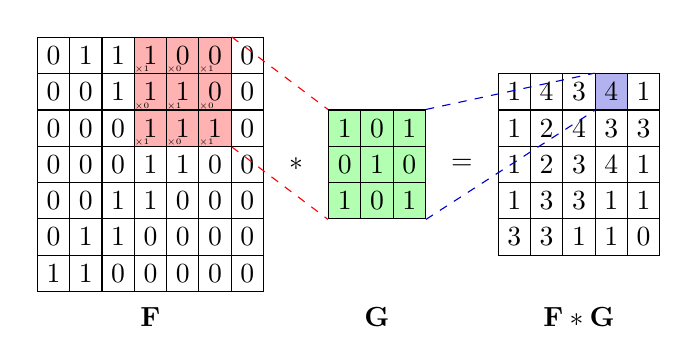
\begin{tikzpicture}[
    2d-arr/.style={matrix of nodes, row sep=-\pgflinewidth, column sep=-\pgflinewidth, nodes={draw}}
  ]

  \matrix (mtr) [2d-arr] {
  0 & 1 & 1 & |[fill=red!30]| 1 & |[fill=red!30]| 0 & |[fill=red!30]| 0 & 0\\
  0 & 0 & 1 & |[fill=red!30]| 1 & |[fill=red!30]| 1 & |[fill=red!30]| 0 & 0\\
  0 & 0 & 0 & |[fill=red!30]| 1 & |[fill=red!30]| 1 & |[fill=red!30]| 1 & 0\\
  0 & 0 & 0 & 1 & 1 & 0 & 0\\
  0 & 0 & 1 & 1 & 0 & 0 & 0\\
  0 & 1 & 1 & 0 & 0 & 0 & 0\\
  1 & 1 & 0 & 0 & 0 & 0 & 0\\
  };

  \node[below=of mtr-5-4] {$\mathbf F$};

  \node[right=0.2em of mtr] (str) {$*$};

  \matrix (K) [2d-arr, right=0.2em of str, nodes={draw, fill=green!30}] {
    1 & 0 & 1 \\
    0 & 1 & 0 \\
    1 & 0 & 1 \\
  };
  \node[below=of K-3-2] {$\mathbf G$};

  \node[right=0.2em of K] (eq) {$=$};

  \matrix (ret) [2d-arr, right=0.2em of eq] {
  1 & 4 & 3 & |[fill=blue!80!black!30]| 4 & 1\\
  1 & 2 & 4 & 3 & 3\\
  1 & 2 & 3 & 4 & 1\\
  1 & 3 & 3 & 1 & 1\\
  3 & 3 & 1 & 1 & 0\\
  };
  \node[below=of ret-4-3] {$\mathbf{F * G}$};

  \draw[dashed, red] (mtr-1-6.north east) -- (K-1-1.north west);
  \draw[dashed, red] (mtr-3-6.south east) -- (K-3-1.south west);

  \draw[dashed, blue!80!black] (K-1-3.north east) -- (ret-1-4.north west);
  \draw[dashed, blue!80!black] (K-3-3.south east) -- (ret-1-4.south west);

  \foreach \i in {1,2,3} {
      \foreach \j in {4,5,6} {
          \node[font=\tiny, scale=0.6, shift={(-1.2ex,-2ex)}] at (mtr-\i-\j) {$\times \pgfmathparse{int(mod(\i+\j,2))}\pgfmathresult$};
        }
    }

\end{tikzpicture}
\caption{Example Convolution}
\label{fig: convolution matrix}
    Figure based on a post by Riebesell. \cite{riebesell_convolution_2022}
\end{figure}
In convolutional neural networks, matrices of weights called kernels or filters replace singular weights in dense layers.
The output of the convolutional layer consists of feature maps, each representing the result of applying one filter to the input data.
These maps capture different aspects such as edges or textures.
A convolutional layer has two other variables: the number and size of filters and the activation function.
The terms stride and padding are used to describe the movement of the filter and the preservation of information on the edge of an input, respectively.
In the figure \ref{fig: convolution matrix}, you can see a filter of size 3x3, which is applied to a 7x7 matrix, with a stride of 1 and no padding, which results in a 5x5 matrix.
The stride determines the number of steps the filter takes between convolutions, with a larger stride resulting in a smaller filter map and less detail.
Padding is an optional parameter that helps to maintain information on the edge of an input and preserve the scale of a picture.

\subsubsection{Pooling Layer}
Pooling is an often used concept in Convolutional Neural Networks to reduce the size of the individual feature map produced by the convolutional layer, while conserving important details of the feature map.
Especially to produce an output which has a similar size as the input, a pooling layer can be avoided \cite{jain_supervised_2007}.
There are multiple types of pooling operations, but the most used ones are Max-Pooling as seen in figure \ref{fig: Max Pooling} and Average-Pooling seen in figure \ref{fig: Average Pooling}.
Which operation is best depends on the type of data to be analysed and its pooling cardinality, which describes the number of extracted features.
There can be said, for smaller cardinalities a Max-Pooling should be used, for larger ones Average-Pooling \cite{boureau_theoretical_2010}.
In the complex layer terminology \cite{goodfellow_deep_2016} there are, the convolution stage, the detector stage (Which is just the usage of a nonlinear activation function) and the pool stage, these stages are sublayers of the large convolutional layer.
In the simple layer terminology, those three are all individual layers.
\begin{figure}[h]
\centering
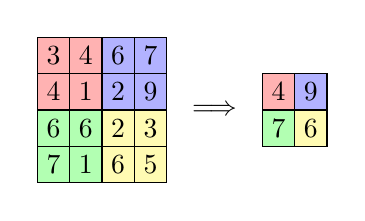
\begin{tikzpicture}[
    2d-arr/.style={matrix of nodes, row sep=-\pgflinewidth, column sep=-\pgflinewidth, nodes={draw}}
  ]

  \matrix (mtr) [2d-arr] {
  |[fill=red!30]| 3 & |[fill=red!30]| 4 & |[fill=blue!30]| 6 & |[fill=blue!30]| 7\\
  |[fill=red!30]| 4 & |[fill=red!30]| 1 & |[fill=blue!30]| 2 & |[fill=blue!30]| 9\\
  |[fill=green!30]| 6 & |[fill=green!30]| 6 & |[fill=yellow!30]| 2 & |[fill=yellow!30]| 3\\
  |[fill=green!30]| 7 & |[fill=green!30]| 1 & |[fill=yellow!30]| 6 & |[fill=yellow!30]| 5\\
  };

  \node[right=0.2em of mtr] (str) {$\Longrightarrow$};

  \matrix (K) [2d-arr, right=0.2em of str] {
    |[fill=red!30]| 4 & |[fill=blue!30]| 9 \\
    |[fill=green!30]| 7 & |[fill=yellow!30]| 6 \\
  };

\end{tikzpicture}
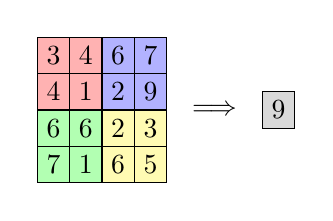
\begin{tikzpicture}[
    2d-arr/.style={matrix of nodes, row sep=-\pgflinewidth, column sep=-\pgflinewidth, nodes={draw}}
  ]

  \matrix (mtr) [2d-arr] {
  |[fill=red!30]| 3 & |[fill=red!30]| 4 & |[fill=blue!30]| 6 & |[fill=blue!30]| 7\\
  |[fill=red!30]| 4 & |[fill=red!30]| 1 & |[fill=blue!30]| 2 & |[fill=blue!30]| 9\\
  |[fill=green!30]| 6 & |[fill=green!30]| 6 & |[fill=yellow!30]| 2 & |[fill=yellow!30]| 3\\
  |[fill=green!30]| 7 & |[fill=green!30]| 1 & |[fill=yellow!30]| 6 & |[fill=yellow!30]| 5\\
  };

  \node[right=0.2em of mtr] (str) {$\Longrightarrow$};

  \matrix (K) [2d-arr, right=0.2em of str] {
    |[fill=gray!30]| 9\\
  };
\end{tikzpicture}
\caption{Max Pooling}
\label{fig: Max Pooling}
Left: Max Pooling, Filter: (2,2) Stride: 2 Right: Max Global Pooling
\end{figure}
\begin{figure}[h]
\centering
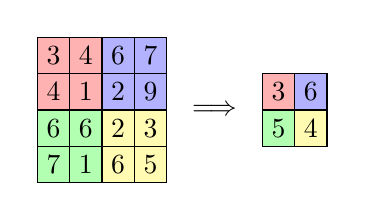
\begin{tikzpicture}[
    2d-arr/.style={matrix of nodes, row sep=-\pgflinewidth, column sep=-\pgflinewidth, nodes={draw}}
  ]

  \matrix (mtr) [2d-arr] {
  |[fill=red!30]| 3 & |[fill=red!30]| 4 & |[fill=blue!30]| 6 & |[fill=blue!30]| 7\\
  |[fill=red!30]| 4 & |[fill=red!30]| 1 & |[fill=blue!30]| 2 & |[fill=blue!30]| 9\\
  |[fill=green!30]| 6 & |[fill=green!30]| 6 & |[fill=yellow!30]| 2 & |[fill=yellow!30]| 3\\
  |[fill=green!30]| 7 & |[fill=green!30]| 1 & |[fill=yellow!30]| 6 & |[fill=yellow!30]| 5\\
  };

  \node[right=0.2em of mtr] (str) {$\Longrightarrow$};

  \matrix (K) [2d-arr, right=0.2em of str] {
    |[fill=red!30]| 3 & |[fill=blue!30]| 6 \\
    |[fill=green!30]| 5 & |[fill=yellow!30]| 4 \\
  };

\end{tikzpicture}
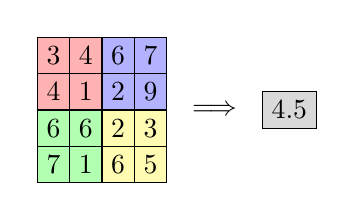
\begin{tikzpicture}[
    2d-arr/.style={matrix of nodes, row sep=-\pgflinewidth, column sep=-\pgflinewidth, nodes={draw}}
  ]

  \matrix (mtr) [2d-arr] {
  |[fill=red!30]| 3 & |[fill=red!30]| 4 & |[fill=blue!30]| 6 & |[fill=blue!30]| 7\\
  |[fill=red!30]| 4 & |[fill=red!30]| 1 & |[fill=blue!30]| 2 & |[fill=blue!30]| 9\\
  |[fill=green!30]| 6 & |[fill=green!30]| 6 & |[fill=yellow!30]| 2 & |[fill=yellow!30]| 3\\
  |[fill=green!30]| 7 & |[fill=green!30]| 1 & |[fill=yellow!30]| 6 & |[fill=yellow!30]| 5\\
  };

  \node[right=0.2em of mtr] (str) {$\Longrightarrow$};

  \matrix (K) [2d-arr, right=0.2em of str] {
    |[fill=gray!30]| 4.5\\
  };

\end{tikzpicture}
\caption{Average Pooling}
\label{fig: Average Pooling}
Left: Average Pooling, Filter: (2,2) Stride: 2 Right: Average Global Pooling
\end{figure}

Now, with the usage of the convolutional layer and the pooling layer, we can preprocess data to get better results with the dense layers, which we still need to classify our data.


\section{Neural Network Testing}\label{sec:neural-network-testing}
The testing methods can be categorized into two distinct categories, which are akin to testing in conventional software.
They are coverage criteria and test case generation.
In the subsequent section, we shall examine various methodologies employed for testing singular deep neural networks \cite{huang_survey_2020}.
But first, how do we define an erroneous behaviour of a neural network, as defined in the equation \ref{eq: erroneous behaviour}?
Where $f: \mathbb{R}^{s_1} \to \mathbb{R}^{s_K}$ is a trained neural network, $\mathcal{H}: \mathbb{R}^{s_1} \to \mathbb{R}^{s_K}$ and a legitimate input $x \in \mathbb{R}^{s_1}$, then we define the erroneous behaviour as:
\begin{equation}
    \arg \max_{j} f_j (x) \neq \arg \max_{j} \mathcal{H}_j (x)
    \label{eq: erroneous behaviour}
\end{equation}

\subsection*{Coverage Criteria}\label{subsec:coverage-criteria}
We need the coverage criteria to get a quantitative basis for deciding how thoroughly our neural network is tested and to ensure that in our network key aspects aren't overlooked.
The criteria used in neural network testing differ from those in software testing.

\subsubsection{Neuron Coverage}
Neuron coverage is the most basic coverage criteria, it is the ratio of the number of neurons activated by the test cases to the total number of neurons in the network \cite{pei_deepxplore_2017}.
A neuron is activated if the output of the neuron is greater than zero.
The neuron coverage is equivalent to the statement coverage in software testing, it helps to measure the thoroughness of the test cases.

\subsubsection{Safety Coverage}
The Safety Coverage is derived, by discretizing the input space into a set of hyper-rectangles \cite{beyer_feature-guided_2018}, each of these hyper-rectangles exhibit the same pattern of activations of neurons, because it has a similar feature set.
A hyper-rectangle is considered safely covered if a test case is classified correctly for all points in the hyper-rectangle.
\subsubsection{Modified Condition/Decision Coverage}
Modified Condition/Decision Coverage (MC/DC) is a method in software testing \cite{hayhurst_practical_2001}, which requires that each condition in a decision is tested independently and that each condition is shown to affect the decision outcome independently.
This is done by varying the input of the condition while holding the other conditions constant \cite{sun_deepconcolic_2019}.
The method is particularly useful in identifying cases where multiple conditions contribute to a decision's outcome.
By using a sign change and a value change to change, it's tried to exploit the relationship between those and use these as a coverage criterion.
\subsubsection{Quantitative Projection}
Quantitative Projection Coverage, is based on the assumption that the input differs on some kind of operation condition \cite{cheng_manifesting_2018}.
For example, for self-driving cars: weather, landscape or impeding items.

\subsection*{Test Case Generation}
But how do we now generate our test case, to get some useful information?
We have, of course, multiple methods to generate our test cases:

\subsubsection{Input Mutation}
Input Mutation, is a method where we take one of the inputs and transform it, by some predefined rules, to generate our test cases .
For example, in combination with safety coverage, we try to mutate the input in that way so that we cover every hyper-rectangle.
\subsubsection{Fuzzing}
Fuzzing, is a method where we generate random inputs, which are modified from the input set, those are then fed into the network \cite{beyer_feature-guided_2018}.
There by, we try to cover as much of the input space as possible.
This can help us because a neural network, is designed for high-dimensional data, aim is to find cases where these small changes to the input cause the DNN to fail or behave unexpectedly.

\subsubsection{Symbolic Execution}
Despite the efficacy of input mutation and fuzzing in generating a substantial quantity of random data, it is uncertain whether certain test objectives will be fulfilled.
With Symbolic Execution, we try to find out which input causes a part of a program to execute.
One approach in Symbolic Execution is concolic testing, which is a hybrid testing technique which is adapted for neural networks with DeepConcolic \cite{sun_deepconcolic_2019}.
Concolic testing combines the concrete execution of a program, with random input generation, hence symbolic data.
There by, the findings of the first step are used to generate the second set of inputs.

\section{Spectrum-Based Fault Localization}\label{sec:spectrum-analysis}
Another important detail that requires introduction, Spectrum-Based Fault Localization (SBFL) \cite{wong_handbook_2023}, it is a technique to identify the source of faults in software.
The term spectrum, describes in this context the execution profile of the program, which is collected during the execution of a test suite.
During the execution, the coverage of each statement by a test case is recorded and if this test case is a success or a failure.
\begin{table}
\centering
\begin{tabular}{|c|c|c|c|}
\hline
\multicolumn{2}{|c|}{} & \multicolumn{2}{c|}{\textbf{Is the statement covered?}}\\
\cline{3-4}
\multicolumn{2}{|c|}{} & \textbf{Yes (1)} & \textbf{No (0)}  \\ \hline
\multirow{2}{*}{\textbf{Execution result}} & \textbf{Failed (0)} &$a_{ef}$ & $a_{nf}$\\
 & \textbf{Successful (1)} & $a_{es}$ & $a_{ns}$\\ \hline
\end{tabular}
\caption{Symbols used in coefficients}
\label{tab: Sus symbols}
\end{table}
SBFL records not only failed test cases but also successful ones.
This provides information on the contrast between failure and success, aiding in the identification of truly faulty statements.
For example, in the first case, code that is often executed or every time, would be marked faulty simply for being in a programme.
In the second case, the code wouldn't be marked faulty because it is also executed frequently in successful test cases.
The term “code coverage” is frequently referred to as “executable statement hit spectrum” (ESHS), which denotes the extent to which certain components of the program under testing have been covered during execution.
Some popular ESHS-based are based on a similarity coefficient, for example Tarantula \cite{jones_empirical_2005} as seen in equation \ref{eq: tarantula} , Ochiai \cite{ochiai_zoogeographical_1957} seen in equation \ref{eq: ochiai} or Dstar \cite{wong_dstar_2014} in equation \ref{eq: dstar} (Often also called $D^*$, where $*$ denotes the used exponent).
\begin{equation}
    \frac{\frac{a_{ef}}{a_{ef} + a_{nf}}}{\frac{a_{ef}}{a_{ef} + a_{nf}}+\frac{a_{es}}{a_{es} + a_{ns}}}
    \label{eq: tarantula}
\end{equation}
\begin{equation}
    \frac{a_{ef}}{\sqrt{(a_{ef}+a_{nf})\cdot(a_{ef}+a_{es})}}
    \label{eq: ochiai}
\end{equation}
\begin{equation}
    \frac{{a_{ef}}^*}{a_{es}+a_{nf}}
    \label{eq: dstar}
\end{equation}
By the work of Lee et al. \cite{hua_jie_lee_study_2009} the formula for Tarantula could even be more simplified like seen in equation \ref{eq: erroneous behaviour}.
Yoo et al. \cite{yoo_human_2017} showed that using genetic programming to create ranking metrics can consistently exceed many human-designed ranking metrics, like the measures discussed before.
\begin{equation}
    \frac{a_{ef}}{a_{ef}+a_{es}}
    \label{eq: simple_tarantula}
\end{equation}
In the following, you can see an Example from Parsa et al. \cite{parsa_software_2023} to see what spectrum analysis is, and what a pitfall of this method is.
The Listing \ref{lst:code_snippet sfl} depicts some simple calculation program, which takes the two integers a and b as input and an integer c for the branching of the calculation.
At line 11, the Max value is wrongly set, this is the fault that needs to be found.
In the Table \ref{tab: sfl}, you can see the suspiciousness values calculated with ochiai and tarantula.

But because line 8, is always executed with line 11 and is overall less executed than line 11, it is the more suspicious statement.
Hence, we can see that spectrum analysis isn't the silver bullet, for eradicating faults in programs, but it can still be a useful tool to reduce the search space for the fault.
\begin{lstlisting}[caption={Example code snippet}, label={lst:code_snippet sfl}]
int getImpact()
{
    scanf("%d %d %d", &a, &b, &c);
    Impact = 0;
    Division = 1;
    Sum = a + b;
    if ((a > 0) && (b > 0))
        Division = a / b;
    Max = b;
    if (a > b)
        Max = b; // Correct: Max = a;
    if (c == 1)
        Impact = Sum;
    if (c == 2)
        Impact = Division;
    if (c == 3)
        Impact = Max;
    return Impact;
}
\end{lstlisting}
\begin{table}[!h]
\centering
\begin{tabular}{|c|c|c|c|c|}
\hline
Line & $a_{es}$ & $a_{ef}$ & Tarantula & Ochiai \\
\hline
6 & 6 & 6 & 0.5 & 0.71 \\
7 & 6 & 6 & 0.5 & 0.71 \\
8 & 2 & 6 & 0.75 & 0.87 \\
9 & 6 & 6 & 0.5 & 0.71 \\
10 & 6 & 6 & 0.5 & 0.71 \\
11 & 3 & 6 & 0.67 & 0.81 \\
12 & 6 & 6 & 0.5 & 0.71 \\
13 & 1 & 0 & 0.0 & 0.0 \\
14 & 6 & 6 & 0.5 & 0.71 \\
15 & 2 & 0 & 0.0 & 0.0 \\
16 & 6 & 6 & 0.5 & 0.71 \\
17 & 3 & 6 & 0.67 & 0.81 \\
18 & 6 & 6 & 0.5 & 0.71\\
\hline
\end{tabular}
\caption{Fault values, for code snippet}
\label{tab: sfl}
\end{table}

There are even more similarity coefficients, to an extent which wouldn't be feasible to be covered in this work, for an extensive survey one can refer to the one by Wong et al. \cite{wong_survey_2016}.

There are some other examples of SBFL, which don't use ESHS, for example Program Invariants Hit Spectrum, which the coverage of program invariants.
Those individuals attempt to identify violations of program properties in failed program executions to locate bugs.
Another one would be the Method Calls Sequence Hit Spectrum, which collects information about the sequence of method calls, during a test-case.
\chapter{Related Work}\label{ch:related-work}
In this chapter, we will discuss proposed approaches for repairing neural networks.
These approaches \cite{nakagawa_experience_2023} can be classified into three categories: training-centric, data-centric, and model-centric.

\section{Training-Centric Approaches}\label{sec:training-centric-approaches}
The training centric solution we want to present is AutoTrainer\cite{zhang_autotrainer_2021} an approach to identify varying issues in training vanishing and exploding gradient, dying ReLU oscillating loss and slow convergence.
AutoTrainer first starts training the model and records data on the training like the loss, it then conducts regular analysis to identify possible issues encountered during training.
Upon detecting an issue, the solution scheduler selects an appropriate repair method.
If a problem persists even after trying a solution, the scheduler moves on to the next solution.
This process continues until the issue is resolved, or all solutions are exhausted unsuccessfully.
The solutions that are used are:
\begin{itemize}
    \item Adding Batch Normalization Layers
    \item Substituting Activation Functions
    \item Adding Gradient Clipping
    \item Substituting Initializers
    \item Adjusting Batch Sizes
    \item Adjusting Learning Rates
    \item Substituting Optimizers
\end{itemize}
Another training centric solution is DeepDiagnosis which isn't like AutoTrainer an automatic approach, but more functioning like a debugger.
Hence, it tries to enable the developer to make sound decisions to enhance the training of a DNN .
It monitors the training of the Network and checks for eight error conditions:
\begin{itemize}
    \item Dead Nodes
    \item Saturated Activation Functions
    \item Exploding Tensors
    \item Not increasing Accuracy
    \item Not decreasing Loss
    \item Unchanged Weights
    \item Exploding Gradients
    \item Fading Gradients
\end{itemize}
When these conditions are met, DeepDiagnosis\cite{wardat_deepdiagnosis_2021} makes these findings available to the developer and also provides a recommendation for actionable fixes to the developer.
\section{Data-Centric Approaches}\label{sec:data-centric-approaches}
One data centric approach for the repair of deep neural networks is DeepRepair\cite{yu_deeprepair_2022} which uses a style guided approach to enhance the training data of an DNN. The Idea for this approach is it to mitigate the gap between the training data and the real-world data provided later when the network is in production, which often contains noise patterns.
This is done by the style of guided data augmentation by introducing the noise patterns which are frequently leading to failure.

To make the augmentation more effective, DeepRepair uses a clustering-based method for generating corrupted data, by identifying and grouping similar failure patterns.
There by, it is ensured that the data covers a broader spectrum of potential real-world failure scenarios, enhancing the robustness of the model.

Another data-centric approach is SENSEI\cite{gao_fuzz_2020}, which uses a fuzz testing derived data augmentation approach to bridge the earlier described gap by exposing and mitigating vulnerabilities in DNNs.

\section{Model-Centric Approaches}\label{sec:model-centric-approaches}
There are numerous model-centric approaches developed over the last few years, so we want to present some of them here at this point.
For example, Apricot\cite{zhang_apricot_2019}, a weight-adaption approach to fix deep learning models (DLM) iteratively.
This is accomplished by leveraging insights from reduced deep learning models (rDLMs) trained on subsets of the original dataset.The approach is based on two main principles: firstly, smaller data sets help to retain the features that are essential for correct classification, and secondly, a set of rDLMs can, on average, classify test cases more accurately than a single model.
Apricot generates the rDLMs and categorizes them based on their performance of specific test cases.
Based on the correctly working rDLMs the average weights are used to correct the weights of the complete DLM toward the weights of the correctly classifying rDLMs or away from the misclassifying rDLMs.

Another approach is NeuRecover\cite{tokui_neurecover_2022}, which tries to resolve an issue which often happens with retraining DNNs. Regression, which means, that if we try to address specific issues to enhance the performance of the models or its areas, it causes a performance decrease in other areas of the model.
NeuRecover is attempting to leverage the training history to identify which parameters should be adjusted, there by aiming to reduce regression.
It firstly aggregates the locations of the faults in the network and by using the training history, attempts to make the smallest necessary adjustment, there by considering the dynamic nature of the network.

Finally, we introduce Arachne\cite{sohn_arachne_2023}, a search-based approach for repairing DNNs by identifying and adjusting the weights that are most likely to cause the targeted misbehavior.
Arachne uses differential evolution to generate patches, which are sets of adjusted neural weights that aim to correct the misclassifications.
The algorithm begins with a group of potential solutions and evolves them over several generations towards greater fitness, as determined by a defined fitness function.
In Arachne, the fitness function plays a critical role in guiding the search process.
It assesses candidate patches based on their ability to correct misclassifications while maintaining correct classifications.
This function strikes a balance between the need to correct errors and the need to maintain the overall accuracy of the model.
Some evolutions of the Search-based approach are DistrRep\cite{calsi_distributed_2023}, which tries to handle multiple misclassifications at the same time, in contrast to the single misclassification handled by Arachne.
Another one is AdRep\cite{li_calsi_adaptive_2023}, this approach tries to overcome the static view of the DNN which is seen in Arachne.

\section{DeepFault}\label{sec:deepfault}
DeepFault\cite{eniser_deepfault_2019} is a white-box testing approach for neural networks, developed by Eniser et al. which is according to the Authors.
\begin{quote}
    ... the first fault localization-based white-box testing approach for DNNs.
\end{quote}
There are two objectives to the approach, the identification of suspicious neurons, which have undesirable behaviour, where the respective neuron is suspected to lead to an undesirable outcome in the whole network.
And the synthesis of new inputs for the neural network, to specially retrain the (most) suspicious values.

In this First Part, DeepFault is establishing a Hit Spectrum($HS$) \ref{eq:hit_spectrum} for all neurons, which take the form of a tuple.
The input, and output layers are left out because they are considered inherently correct.
\begin{equation}
    HS_n = (attr_n^{as}, attr_n^{af}, attr_n^{ns}, attr_n^{nf})\label{eq:hit_spectrum}
\end{equation}
\begin{itemize}
    \item $attr^{as}_n$ is the number of times the neuron $n$ is activated in successful test cases.
    \item $attr^{af}_n$ is the number of times the neuron $n$ is activated in failed test cases.
    \item $attr^{ns}_n$ is the number of times the neuron $n$ is not activated in successful test cases.
    \item $attr^{nf}_n$ is the number of times the neuron $n$ is not activated in failed test cases.
\end{itemize}
Then the hit spectra are in a suspiciousness measures, in DeepFault Tarantula \ref{eq: tarantula}, Ochiai \ref{eq: ochiai}, $D^3$ \ref{eq: dstar} are used.
These are not used to identify one wrong neuron, but rather a set of wrong neurons.
For that, the suspiciousness values of the neurons are used to sort the neurons in decreasing order of suspiciousness, if multiple neurons happen to get the same value, the neuron in a deeper layer is used.

Guided by the suspiciousness measures, DeepFault modifies the input, for which the neural network has made the correct decision, in a targeted way.
The synthesis task is supported by a gradient ascent algorithm that aims to determine the degree to which an appropriately classified input should and could be modified to enhance the activation values of suspicious neurons.
\chapter{Mutation-Based Accuracy Improvements}\label{ch:mutation-based-accuracy-improvements}
In the following chapter, we describe our approach for our ``mutation-based accuracy improvements'', starting with the adaptation of DeepFault's \cite{eniser_deepfault_2019} spectrum fault localization.
Afterwards, we go through our work and choices for the mutations of a neural network.

\section{Spectrum-based fault localisation}\label{sec:spectrum-based-fault-localisation}
For the Spectrum-based fault localization, we adapted the DeepFault \cite{eniser_deepfault_2023} code to our needs.
Especially, we adapted the functions to the recent versions of the used libraries and added some additional functions to save and load the data.

%todo: rework this paragraph
The functions adapted from the DeepFault paper are now invoked in the \texttt{run\_analysis} \ref{lst:main analysis} function, which is the main function for the analysis, to ease the use of the analysis.
The function manages the model loading and the experiment or working paths.
The program checks if the necessary data, such as classifications, layer outputs, or spectrum matrices, is already available before executing the analysis functions and saving the outputs.
The network's neuron count is aggregated, and if the number of selected neurons \texttt{susp\_num} is less than the number of modifiable neurons, the \texttt{susp\_num} most suspicious neurons are returned.
Otherwise, all modifiable neurons are returned, ranked by their level of suspicion.
To determine the suspiciousness, we use the $\text{D}^*$, Tarantula, and Ochiai methods.
The option to return a specified number of random neurons has also been included \ref{lst:random_choosing}.
The function returns a list of tuples in the format of $(layer, layer\_index)$, ranked by relevance.

\lstinputlisting[language=Python, linerange={8-64}, caption={Main analysis function}, label={lst:main analysis}]{source_analysis/__init__.py}
\lstinputlisting[language=Python, linerange={59-71}, caption={Random Choosing, of neurons}, label={lst:random_choosing}]{source_analysis/analysis.py}

The saving and loading functions \ref{lst:saving} required adaptation due to the depreciation of the \texttt{.value} property in h5py \cite{collette_h5pyh5py_2022}.
Therefore, every loading function needs to use indexing instead of the property used by the old DeepFault code.
Save and load functions were added for the spectrum matrices and ranked neurons.
These functions are constant since the analysis is only executed once at the start of the algorithm before any model modifications are made.
This improves execution times by preventing multiple executions.

\lstinputlisting[language=Python, linerange={19-81,90-123,154-195}, caption={Saving and loading data}, label={lst:saving}]{source_analysis/utilities.py}

Additionally, we modified the \texttt{get\_layer\_outs} function as shown in listing \ref{lst:layer outs} from native Keras \cite{chollet_keras_2015} calls to TensorFlow \cite{martin_abadi_tensorflow_2015} via \texttt{tf.keras}, which uses Keras as its backend, as recommended by the release notes of Keras 2.13.0. .
Because of its better integration with the rest of the TensorFlow library.

\lstinputlisting[language=Python, linerange={82-87}, caption={Layer outs}, label={lst:layer outs}]{source_analysis/utilities.py}

The \texttt{construct\_spectrum\_matrices} function as shown in listing \ref{lst:spectrum matrice} has been modified to use \texttt{enumerate} in the loops, allowing for the value and index to be obtained in a single loop.
This modification has resulted in a reduction in the function's runtime.

\lstinputlisting[language=Python, linerange={56-90}, caption={Construct spectrum matrice}, label={lst:spectrum matrice}]{source_analysis/test_network.py}

\section{Mutation of the neural network}\label{sec:mutation-of-the-neural-network}
Now we move on to the second step in our approach: modifying our network.
We designed the function \texttt{run\_modification\_algorithm} in listing \ref{lst:mutation} and schematically shown in \ref{fig:flowchart} for this purpose.
Our model and the associated dataset are used, along with a chosen similarity coefficient and modification function.
In addition, we can specify whether to train the model and set an offset for the loss and accuracy.
We can also indicate if we intend to regress the loss and accuracy, which is used as a break condition.
The four break conditions that were introduced require both loss and accuracy to be compared and both to break, or one of them to break, if we want to compare each individually, we can also just compare one individually.
At line 15, \texttt{tf.random.set\_seed(42)} is included for evaluation purposes, to enable comparison of results from different runs.

The evaluation process utilises certain values that are not required in production code.
The \texttt{run} parameter, which simply sets the name of the data analysis run to distinguish between different runs.
In addition, we introduced \texttt{old\_loss} and \texttt{old\_accuracy} to save time by outsourcing the initial model evaluation.
This evaluation is necessary at the start of the function and now only needs to be performed once, rather than every time the function is used.
The pandas functions are also included to gather evaluation data.

\lstinputlisting[language=Python, linerange={9-58}, caption={Modification Algorithm}, label={lst:mutation}]{source_mutation/__init__.py}
\begin{figure}[h]
    \centering
    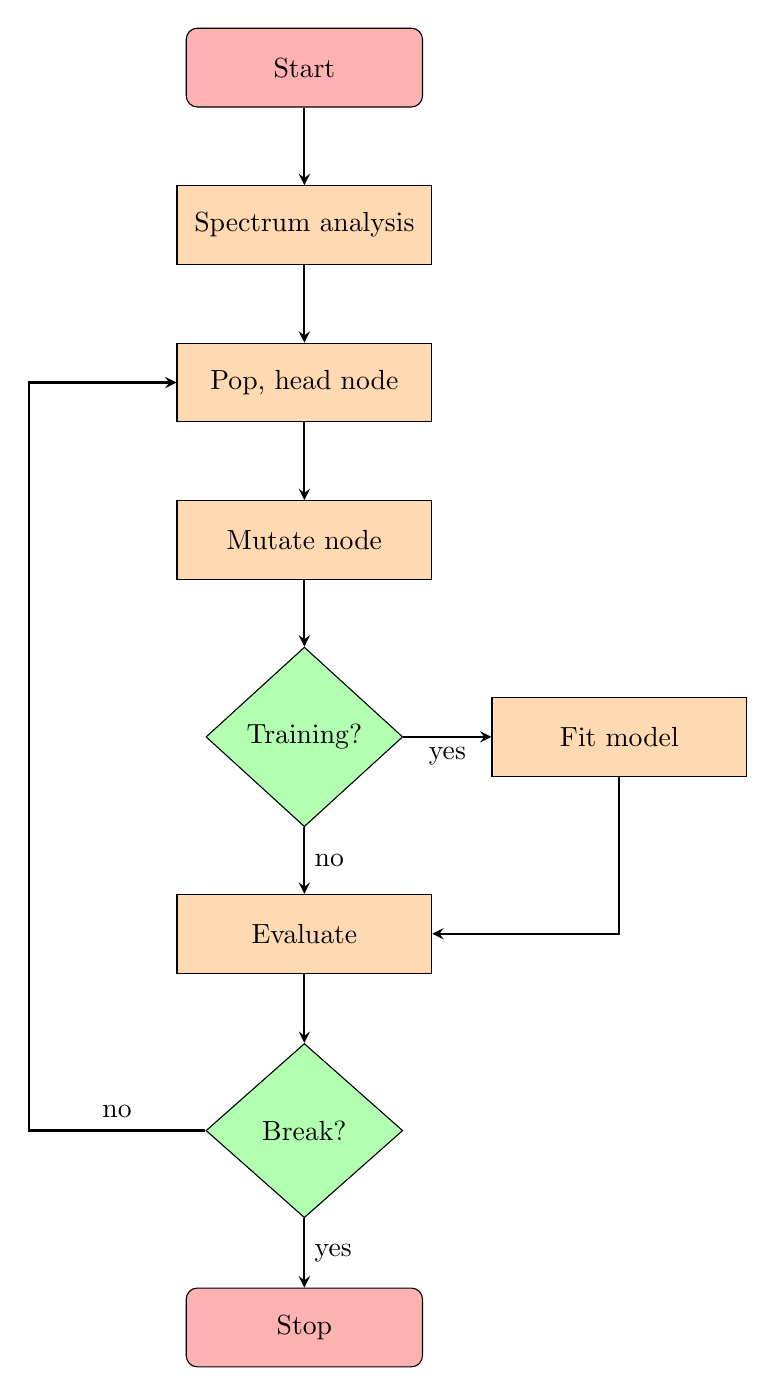
\begin{tikzpicture}[node distance=2cm]
        \node (start) [startstop] {Start};
        \node (pro1) [process, below of=start] {Spectrum analysis};
        \node (pro2) [process, below of=pro1] {Pop, head node};
        \node (pro3) [process, below of=pro2] {Mutate node};
        \node (dec1) [decision, below of=pro3, yshift=-0.5cm] {Training?};
        \node (pro4a) [process, below of=dec1, yshift=-0.5cm] {Evaluate};
        \node (pro4b) [process, right of=dec1, xshift=2cm] {Fit model};
        \node (dec2) [decision, below of=pro4a, yshift=-0.5cm] {Break?};
        \node (stop) [startstop, below of=dec2, yshift=-0.5cm] {Stop};

        \draw [arrow] (start) -- (pro1);
        \draw [arrow] (pro1) -- (pro2);
        \draw [arrow] (pro2) -- (pro3);
        \draw [arrow] (pro3) -- (dec1);
        \draw [arrow] (dec1) -- node[anchor=north] {yes} (pro4b);
        \draw [arrow] (pro4b) |- (pro4a);
        \draw [arrow] (dec1) -- node[anchor=west] {no} (pro4a);
        \draw [arrow] (pro4a) -- (dec2);
        \draw [arrow] (dec2) -- node[anchor=west] {yes} (stop);
        \draw [arrow] (dec2) -- node[anchor=south, above=1pt] {no} ++(-3.5,0) |- (pro2);
    \end{tikzpicture}
    \caption{Flowchart of the \texttt{run\_modification} algorithm.}
    \label{fig:flowchart}
\end{figure}

Now, let's discuss the mutation functions that we pass to our main function.
These functions allow us to modify the weights and biases of a neuron, which is similar to the theoretical representation of a neuron given in the equation \ref{eq: DenseLayer} the background chapter.
The basic functionality of the mutation functions is mostly the same.
We first isolate the layer from the model, which is the first entry in the coordinate tuple.
As seen in the two listing \ref{lst:weight_mod}, \ref{lst:bias_mod} which are the weight and bias modification functions, respectively.
Then, we obtain the weights, where the first entry represents the weights of the neuron and the second entry represents the biases.
The matrix can be mutated according to specific requirements.
To do this, isolate the entries that represent the specified neuron in the second entry of the coordinate and modify them accordingly.
Finally, reassign the weights back to the layer and return the model, which must then be recompiled.

\lstinputlisting[language=Python, linerange={4-33}, caption={Weight Modification Functions}, label={lst:weight_mod}]{source_mutation/utilities.py}
\lstinputlisting[language=Python, linerange={35-45}, caption={Bias Modification Functions}, label={lst:bias_mod}]{source_mutation/utilities.py}

Multiple mutation functions have been implemented for not only dense layers but also 2D Convolution Layers.
Mutation functions are used to assign a singular value to all weights or the bias of a neuron.
This value can either be fixed or random, derived from a uniform or Gaussian normal distribution.
For random values, each weight value can be assigned a new random number individually.
Additionally, scalar mutation functions in listing \ref{lst:scalar_weight_mod} and \ref{lst:scalar_bias_mod} can modify the existing values without assigning new ones.

\lstinputlisting[language=Python, linerange={68-81,115-127}, caption={Scalar Weight Modification Functions}, label={lst:scalar_weight_mod}]{source_mutation/utilities.py}
\lstinputlisting[language=Python, linerange={87-97}, caption={Scalar Bias Modification Functions}, label={lst:scalar_bias_mod}]{source_mutation/utilities.py}
\chapter{Evaluation and Results}\label{ch:results}
In this chapter, we will discuss the performance of our approach towards neural networks.
We will explore various options available through our approach to elicit optimal results.
To achieve this, the evaluation will be based on the following research questions:
\begin{enumerate}
    \item[]\textbf{RQ1: Impact of Training on Mutated Models} How does training a mutated pre-trained model impact its performance metrics?
    \item[]\textbf{RQ2: Effects of Mutation Without Training} What is the effect on performance metrics when a pre-trained model is mutated without further training?
    \item[]\textbf{RQ3: Effects of the extend of pre Training} What is the effect on performance metrics, depending on how many epochs the model is pre-trained?
    \item[]\textbf{RQ4: Training Dataset Size and Approach Performance} What is the impact of the size of the training dataset on the approach's effectiveness?
    \item[]\textbf{RQ5: Influence of Suspiciousness Measures} How do different suspiciousness measures influence the outcomes of the experiments?
    \item[]\textbf{RQ6: CNN vs. DNN Architectural Efficiency} Which architecture yields better results for our approach: CNN or DNN?
    \item[]\textbf{RQ7: Offset Variations in Loss and Accuracy} How do variations in offset for loss and accuracy affect the approach's performance?
    \item[]\textbf{RQ8: Break Conditions and Algorithm Performance} What is the effect of different break conditions on the efficiency and effectiveness of the algorithm?
    \item[]\textbf{RQ9: Contributions of Different Mutation Functions} How do different mutation functions contribute to the model's performance with our Algorithm?
\end{enumerate}
\section{Setup}\label{sec:setup}

We evaluated our approach on a Workstation consisting of an AMD Ryzen 9 3900X 12-Core Processor 4,6 GHz, with 32 GB of RAM and an NVIDIA GeForce RTX 4070Ti GPU with 12 GB of VRAM and 7680 CUDA Cores.
The setup is running Ubuntu release 22.04, running with Windows Subsystem for Linux, on Microsoft Windows 11 Pro, we use it because since version 2.11\cite{noauthor_build_2023} TensorFlow doesn't support GPU acceleration natively any more.
Regarding the Software, we are using Python version 3.10.12 and using TensorFlow version 2.14.1, with CUDA version 12.3.

\subsection{Architecture}\label{subsec:architecture}
We are using the Fashion-MNIST dataset\cite{xiao_fashion-mnist_2017} for our experiments, which consists of 60,000 training images and 10,000 test images, each of size 28×28 pixels, with 10 classes.
For the evaluation we haven't used not only the whole, but also a half and a quarter of the training data, which are derived from the original training data, by using Scikit-learn's\cite{pedregosa_scikit-learn_2011} \texttt{train\_test\_split} function, with a test size of 0.5 and 0.75 respectively.

We used 2 DNNs and 2 CNNs, in the following table \ref{tab:archi} a plain number describes the number of neurons in a dense layer. $CL$ describes a combination of a convolutional layer with a stride of $(1,1)$ and a kernel size of $(3,3)$ and a pooling layer with a pool size of $(2,2)$. We used.
Adam as our optimizer with a learning rate of 0.001.

The models were selected for their small size and ability to accommodate both deep neural networks and convolutional neural networks.
This was done to save time and allow for the evaluation of as many parameters as possible within the time frame of this thesis.
% Please add the following required packages to your document preamble:
% \usepackage{multirow}
% \usepackage{lscape}
% Please add the following required packages to your document preamble:
% \usepackage{multirow}
\begin{table}[htbp]
    \centering
    \caption{Overview of Neural Network Architectures used for evaluation}
    \begin{tabular}{|c|c|c|}
        \hline
        Model Name            & Mod. Param.         & Architecture                 \\ \hline
        \multirow{2}{*}{DNN1} & \multirow{2}{*}{16} & \multirow{2}{*}{$<16>$}      \\
        &                     &                              \\ \hline
        \multirow{2}{*}{DNN2} & \multirow{2}{*}{64} & \multirow{2}{*}{$<4x16>$}    \\
        &                     &                              \\ \hline
        \multirow{2}{*}{CNN1} & \multirow{2}{*}{12} & \multirow{2}{*}{$<CL,4>$}    \\
        &                     &                              \\ \hline
        \multirow{2}{*}{CNN2} & \multirow{2}{*}{20} & \multirow{2}{*}{$<CL,CL,4>$} \\
        &                     &                              \\ \hline
    \end{tabular}
    \label{tab:archi}
\end{table}
\begin{table}[htbp]
    \centering
    \caption{Results of the initial Training of the different models}
    \begin{tabular}{|cc|ccc|ccc|}
        \hline
        \multicolumn{2}{|c|}{Model} & \multicolumn{3}{c|}{Accuracy} & \multicolumn{3}{c|}{Loss} \\ \hline
        \multicolumn{1}{|c|}{Name}                  & Init. Epochs & \multicolumn{1}{c|}{Full}    & \multicolumn{1}{c|}{Half}    & Quarter & \multicolumn{1}{c|}{Full}    & \multicolumn{1}{c|}{Half}     & Quarter  \\ \hline
        \multicolumn{1}{|c|}{\multirow{2}{*}{DNN1}} & 1              & \multicolumn{1}{c|}{82.84\%} & \multicolumn{1}{c|}{81.49\%} & 78.65\% & \multicolumn{1}{c|}{49.11\%} & \multicolumn{1}{c|}{53.46\%}  & 62.00\%  \\ \cline{2-8}
        \multicolumn{1}{|c|}{}                      & 6              & \multicolumn{1}{c|}{84.23\%} & \multicolumn{1}{c|}{83.76\%} & 83.57\% & \multicolumn{1}{c|}{44.42\%} & \multicolumn{1}{c|}{44.48\%}  & 46.94\%  \\ \hline
        \multicolumn{1}{|c|}{\multirow{2}{*}{DNN2}} & 1              & \multicolumn{1}{c|}{80.46\%} & \multicolumn{1}{c|}{79.20\%} & 75.97\% & \multicolumn{1}{c|}{54.05\%} & \multicolumn{1}{c|}{57.90\%}  & 66.21\%  \\ \cline{2-8}
        \multicolumn{1}{|c|}{}                      & 6              & \multicolumn{1}{c|}{83.52\%} & \multicolumn{1}{c|}{83.04\%} & 82.74\% & \multicolumn{1}{c|}{44.23\%} & \multicolumn{1}{c|}{46.79\%}  & 48.88\%  \\ \hline
        \multicolumn{1}{|c|}{\multirow{2}{*}{CNN1}} & 1              & \multicolumn{1}{c|}{74.34\%} & \multicolumn{1}{c|}{77.31\%} & 42.62\% & \multicolumn{1}{c|}{72.88\%} & \multicolumn{1}{c|}{66.83\%}  & 147.63\% \\ \cline{2-8}
        \multicolumn{1}{|c|}{}                      & 6              & \multicolumn{1}{c|}{83.69\%} & \multicolumn{1}{c|}{82.14\%} & 61.06\% & \multicolumn{1}{c|}{48.44\%} & \multicolumn{1}{c|}{47.35\%}  & 95.61\%  \\ \hline
        \multicolumn{1}{|c|}{\multirow{2}{*}{CNN2}} & 1              & \multicolumn{1}{c|}{70.49\%} & \multicolumn{1}{c|}{54.52\%} & 63.20\% & \multicolumn{1}{c|}{80.13\%} & \multicolumn{1}{c|}{111.68\%} & 100.31\% \\ \cline{2-8}
        \multicolumn{1}{|c|}{}                      & 6              & \multicolumn{1}{c|}{78.43\%} & \multicolumn{1}{c|}{77.37\%} & 74.56\% & \multicolumn{1}{c|}{60.28\%} & \multicolumn{1}{c|}{59.29\%}  & 65.74\%  \\ \hline
    \end{tabular}
    \label{tab:results}
\end{table}
\subsection{Parameters}\label{subsec:parameters}
Fo our evaluation we used the following parameters:
\begin{enumerate}
    \item[]\textbf{Similarity coefficient:} tarantula, dstar with value 3, ochiai and random
    \item[]\textbf{Mutation functions:} \texttt{modify\_weight\_one\_random\_gauss,\\ modify\_weight\_all\_random\_gauss, modify\_bias, modify\_bias\_random\_gauss, modify\_all\_weights, modify\_all\_weights\_by\_scalar,\\modify\_all\_weights\_by\_scalar\_random\_gauss,\\modify\_weight\_all\_random\_by\_scalar\_gauss}
    \item[]\textbf{Break conditions:} loss, accuracy, loss and accuracy, loss or accuracy
    \item[]\textbf{Loss offset:} 0.005, 0
    \item[]\textbf{Accuracy offset:} 0.01, 0
    \item[]\textbf{Loss and accuracy regression:} True for all runs
    \item[]\textbf{Values:} -1, -0.5, 0, 0.5, 1 \textit{0 just for value assignment, basically a deletation of a neuron}
    \item[]\textbf{Sigma for random:} 0.5, 1
\end{enumerate}
\section{Results}\label{sec:results}

\subsection{Impact of Training on Mutated Models}\label{subsec:impact-of-training-on-mutated-models}
In this section, we will discuss the impact of training on mutated models.
Only till 20 Epochs, afterwards 5 epochs for untrained and 10 for trained models.
\begin{figure}
    \centering
    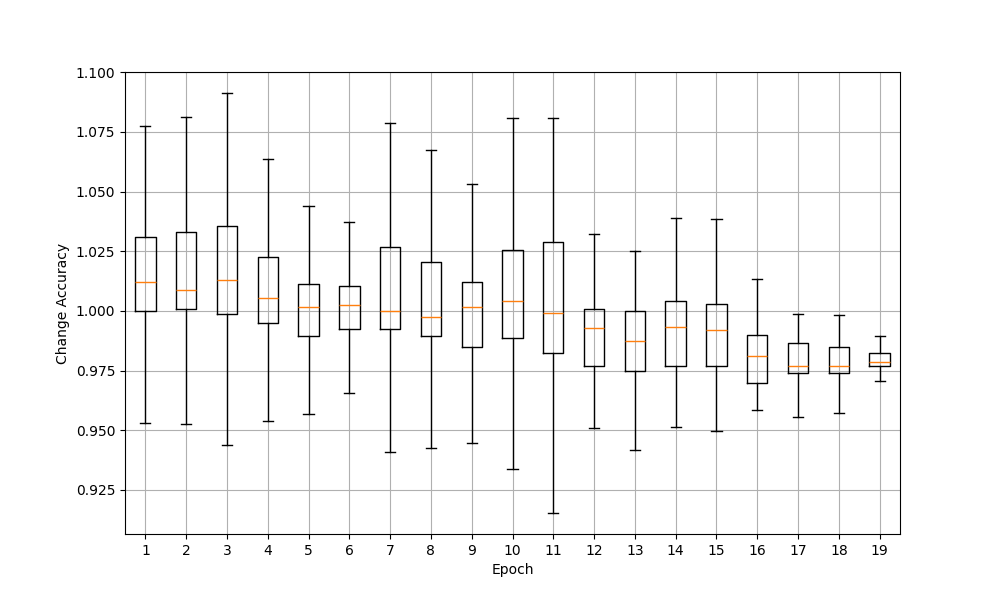
\includegraphics[width=\textwidth]{plots/Trained_Change_Acc.png}
    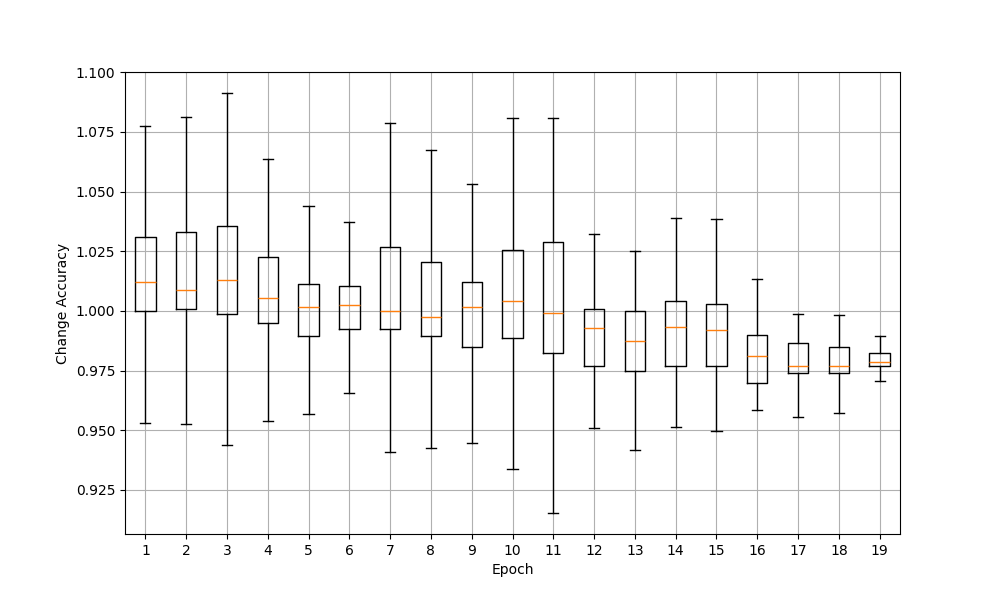
\includegraphics[width=\textwidth]{plots/Trained_Change_Loss.png}
    \caption{Loss and accuracy of the models, with training}
    \label{fig:loss-accuracy-training}
\end{figure}
\begin{figure}
    \centering
    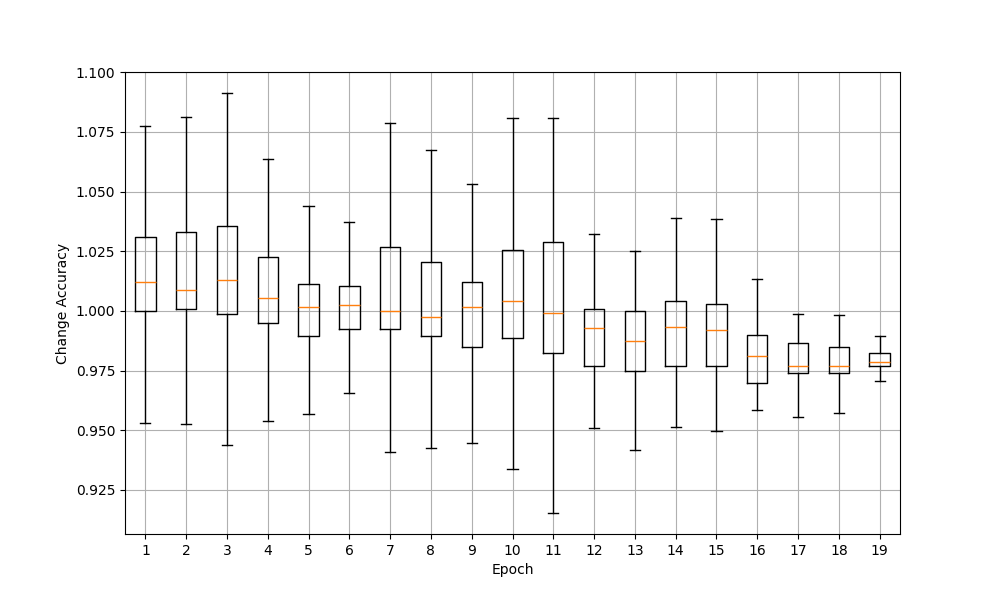
\includegraphics[width=\textwidth]{plots/Trained_Points_perEpoch.png}
    \caption{Decay of data points, per epoch, with training}
    \label{fig:decay_training}
\end{figure}
\subsection{Effects of Mutation Without Training}\label{subsec:effects-of-mutation-without-training}
Only till 20 Epochs, afterwards 5 epochs for untrained and 10 for trained models.
\begin{figure}
    \centering
    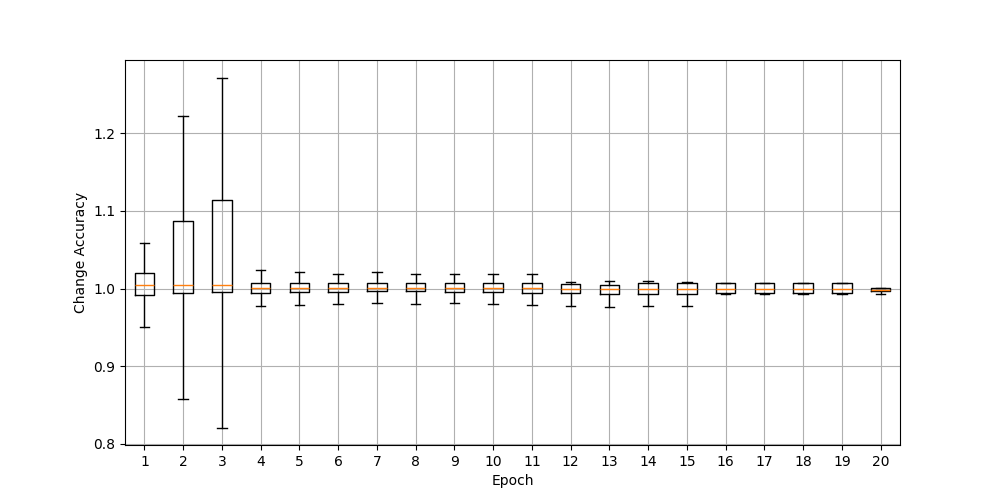
\includegraphics[width=\textwidth]{plots/NotTrained_Change_Acc.png}
    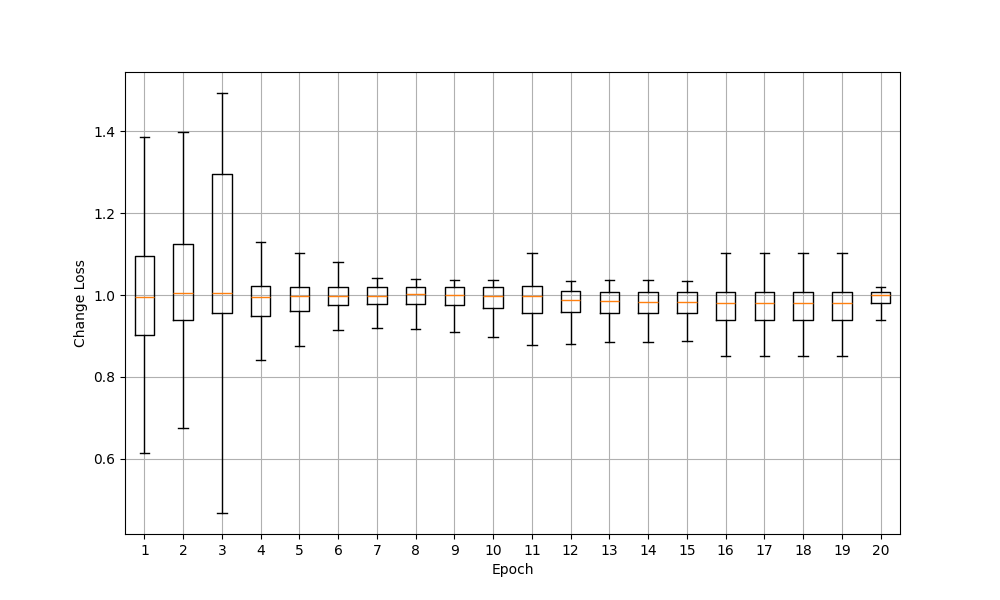
\includegraphics[width=\textwidth]{plots/NotTrained_Change_Loss.png}
    \caption{Loss and accuracy of the models, without training}
    \label{fig:loss-accuracy-Notraining}
\end{figure}
\begin{figure}
    \centering
    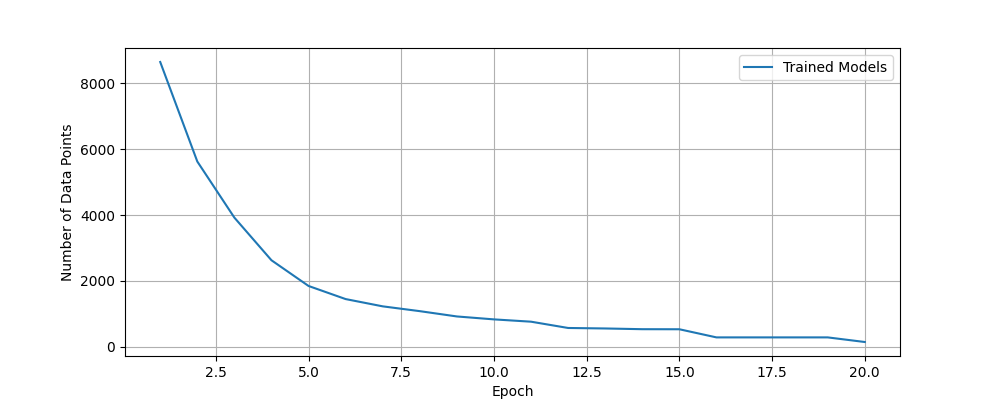
\includegraphics[width=\textwidth]{plots/NotTrained_Points_perEpoch.png}
    \caption{Decay of data points, per epoch, without training}
    \label{fig:decay_Notraining}
\end{figure}
\subsection{Effects of the extend of pre Training}\label{subsec:effects-of-the-extend-of-pre-training}
Because of the bad results for 6 epochs, after that only 1 epoch.
\begin{figure}
    \begin{subfigure}{0.5\textwidth}
        \centering
        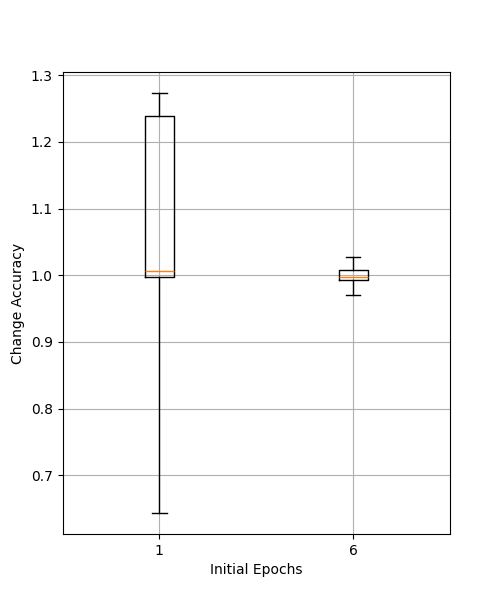
\includegraphics[width=0.95\textwidth]{plots/InitEpoch_NotTrained_accuracy.png}
    \end{subfigure}
    \begin{subfigure}{0.5\textwidth}
        \centering
        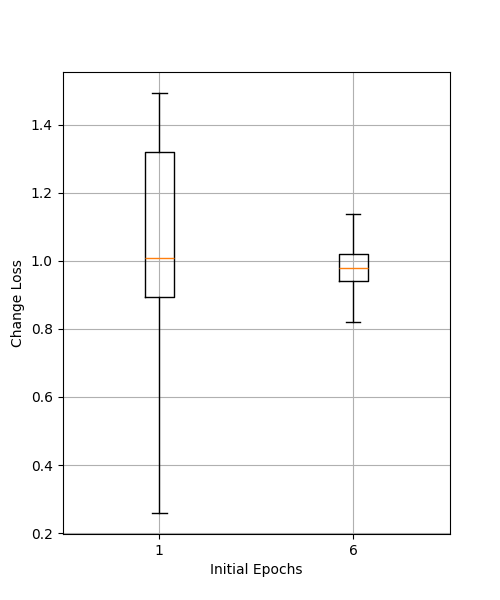
\includegraphics[width=0.95\textwidth]{plots/InitEpoch_NotTrained_loss.png}
    \end{subfigure}
    \caption{Loss and accuracy, without training, with different initial epochs}
    \label{fig:initial-epochs-notraining}
\end{figure}
\begin{figure}
    \begin{subfigure}{0.5\textwidth}
        \centering
        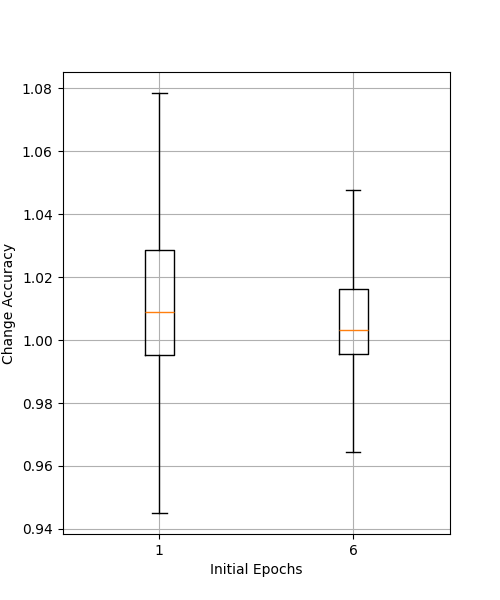
\includegraphics[width=0.95\textwidth]{plots/InitEpoch_Trained_accuracy.png}
    \end{subfigure}
    \begin{subfigure}{0.5\textwidth}
        \centering
        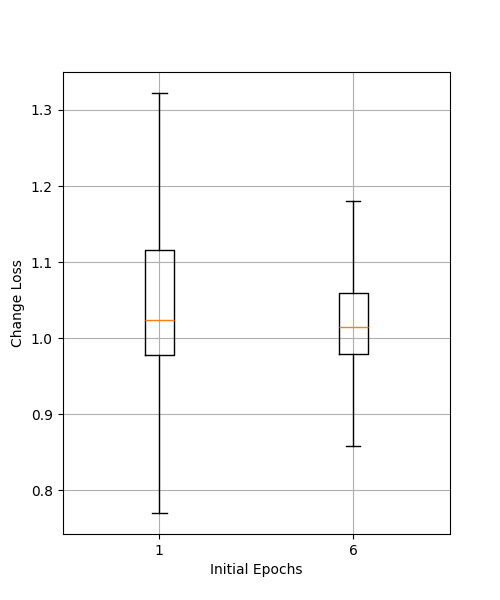
\includegraphics[width=0.95\textwidth]{plots/InitEpoch_Trained_loss.png}
    \end{subfigure}
    \caption{Loss and accuracy, with training, with different initial epochs}
    \label{fig:initial-epochs-training}
\end{figure}
\subsection{Training Dataset Size and Model Performance}\label{subsec:training-dataset-size-and-model-performance}
\begin{figure}
    \begin{subfigure}{0.5\textwidth}
        \centering
        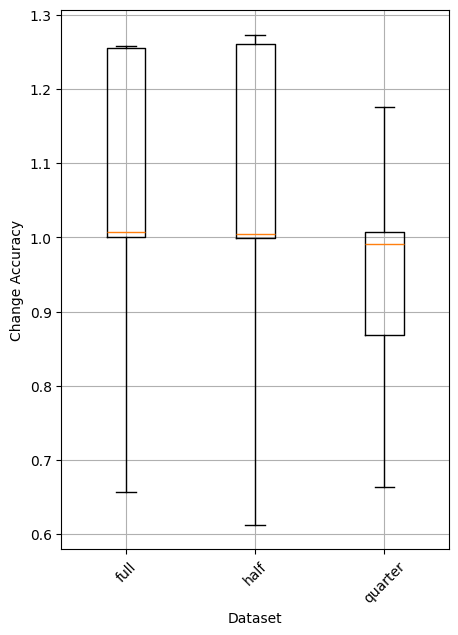
\includegraphics[width=0.95\textwidth]{plots/Dataset_NotTrained_accuracy.png}
    \end{subfigure}
    \begin{subfigure}{0.5\textwidth}
        \centering
        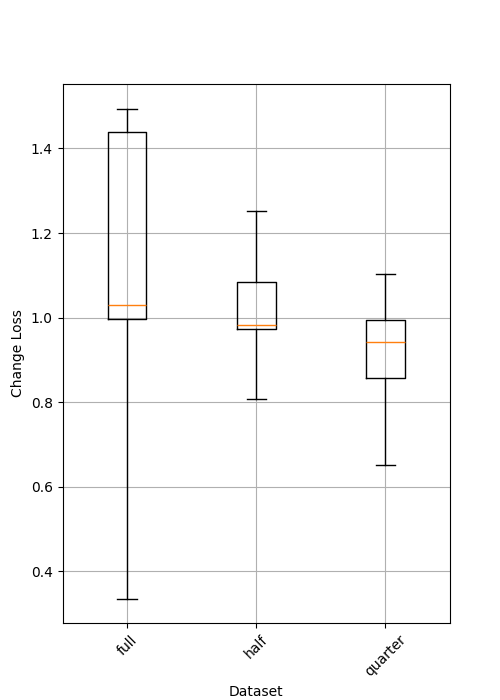
\includegraphics[width=0.95\textwidth]{plots/Dataset_NotTrained_loss.png}
    \end{subfigure}
    \caption{Loss and accuracy, without training, with different dataset sizes}
    \label{fig:dataset-size-notraining}
\end{figure}
\begin{figure}
    \begin{subfigure}{0.5\textwidth}
        \centering
        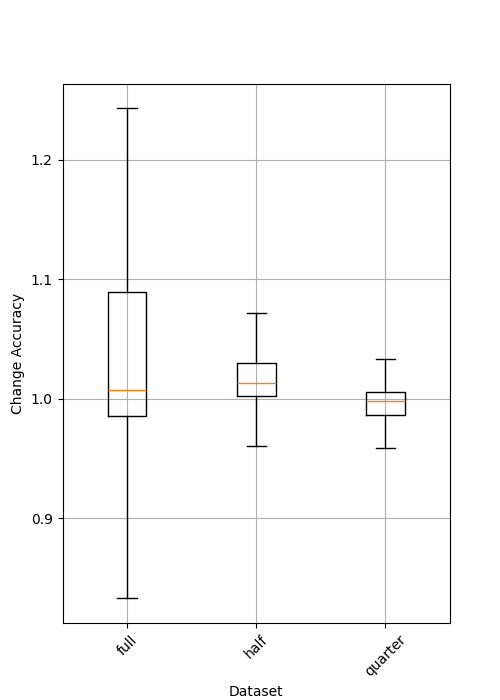
\includegraphics[width=0.95\textwidth]{plots/Dataset_Trained_accuracy.png}
    \end{subfigure}
    \begin{subfigure}{0.5\textwidth}
        \centering
        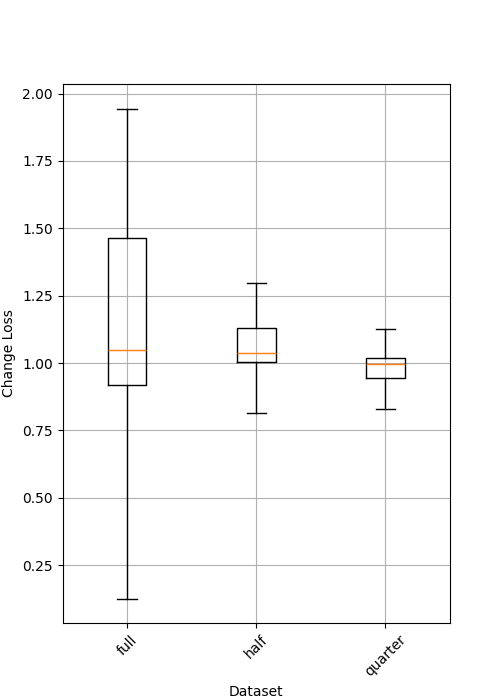
\includegraphics[width=0.95\textwidth]{plots/Dataset_Trained_loss.png}
    \end{subfigure}
    \caption{Loss and accuracy, with training, with different dataset sizes}
    \label{fig:dataset-size-training}
\end{figure}
\subsection{Influence of Suspiciousness Measures}\label{subsec:influence-of-suspiciousness-measures}
\begin{figure}
    \begin{subfigure}{0.5\textwidth}
        \centering
        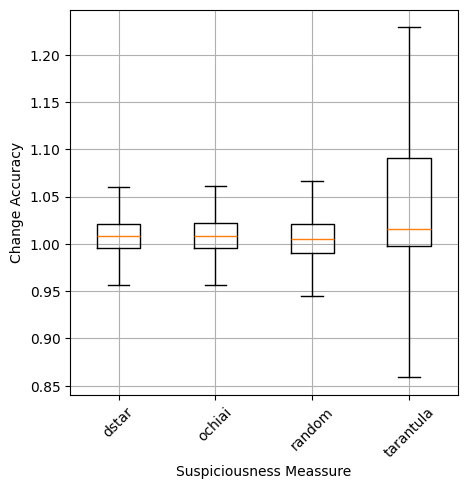
\includegraphics[width=0.95\textwidth]{plots/Meassure_Trained_accuracy.png}
    \end{subfigure}
    \begin{subfigure}{0.5\textwidth}
        \centering
        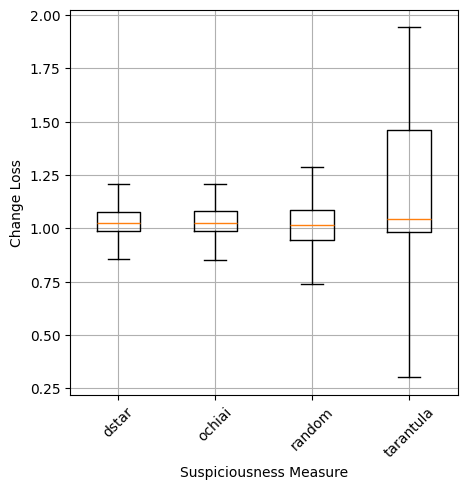
\includegraphics[width=0.95\textwidth]{plots/Meassure_Trained_loss.png}
    \end{subfigure}
    \caption{Loss and accuracy, with training, with different suspiciousness measures}
    \label{fig:suspiciousness-measures-training}
\end{figure}
\begin{figure}
    \begin{subfigure}{0.5\textwidth}
        \centering
        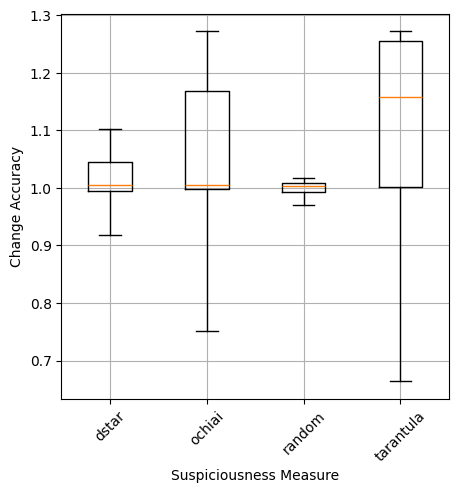
\includegraphics[width=0.95\textwidth]{plots/Meassure_NotTrained_accuracy.png}
    \end{subfigure}
    \begin{subfigure}{0.5\textwidth}
        \centering
        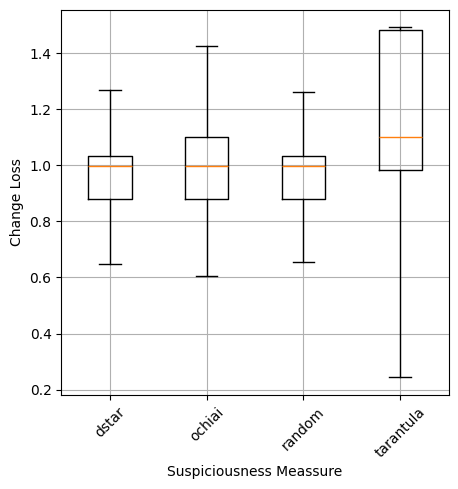
\includegraphics[width=0.95\textwidth]{plots/Meassure_NotTrained_loss.png}
    \end{subfigure}
    \caption{Loss and accuracy, without training, with different suspiciousness measures}
    \label{fig:suspiciousness-measures-notraining}
\end{figure}
\subsection{CNN vs. DNN Architectural Efficiency}\label{subsec:cnn-vs.-dnn-architectural-efficiency}
\begin{figure}
    \begin{subfigure}{0.5\textwidth}
        \centering
        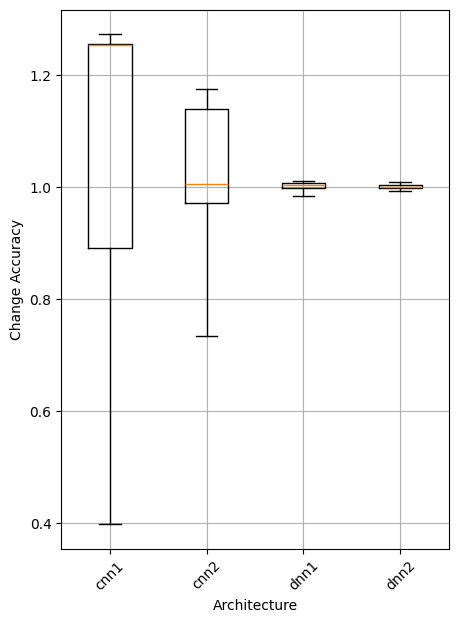
\includegraphics[width=0.95\textwidth]{plots/Architecture_NotTrained_accuracy.png}
    \end{subfigure}
    \begin{subfigure}{0.5\textwidth}
        \centering
        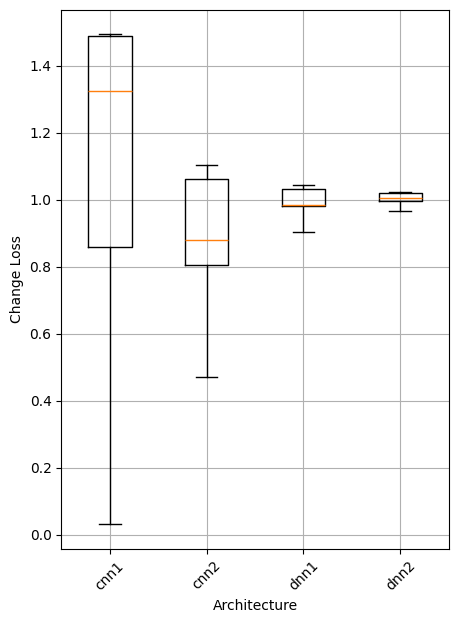
\includegraphics[width=0.95\textwidth]{plots/Architecture_NotTrained_loss.png}
    \end{subfigure}
    \caption{Loss and accuracy, without training, with different architectures}
    \label{fig:architecture-notraining}
\end{figure}
\begin{figure}
    \begin{subfigure}{0.5\textwidth}
        \centering
        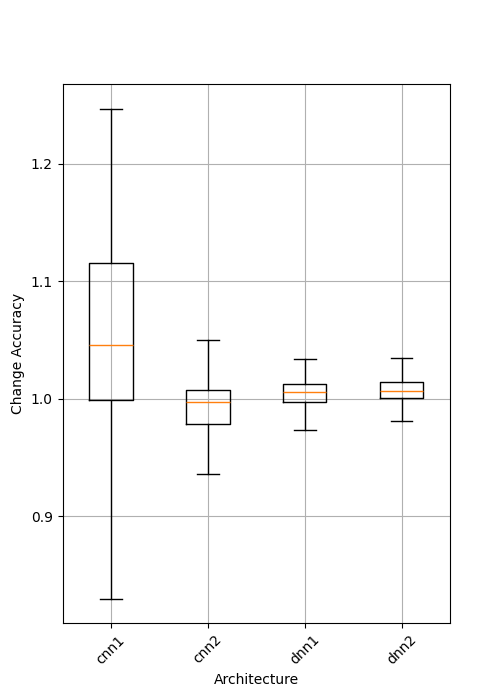
\includegraphics[width=0.95\textwidth]{plots/Architecture_Trained_accuracy.png}
    \end{subfigure}
    \begin{subfigure}{0.5\textwidth}
        \centering
        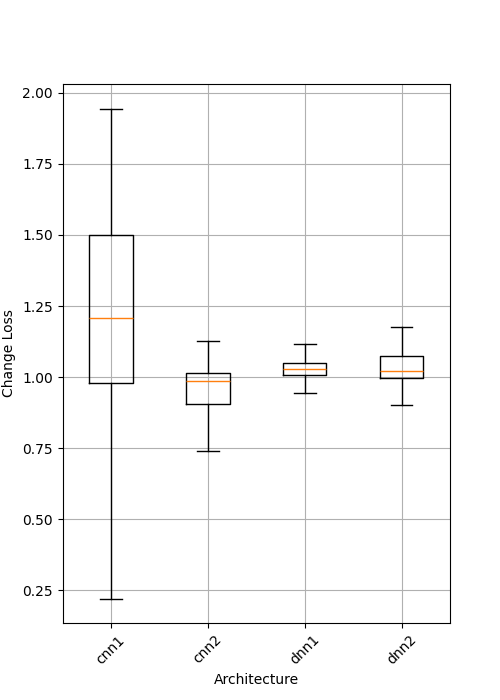
\includegraphics[width=0.95\textwidth]{plots/Architecture_Trained_loss.png}
    \end{subfigure}
    \caption{Loss and accuracy, with training, with different architectures}
    \label{fig:architecture-training}
\end{figure}
\subsection{Offset Variations in Loss and Accuracy}\label{subsec:offset-variations-in-loss-and-accuracy}
\begin{figure}
    \begin{subfigure}{0.5\textwidth}
        \centering
        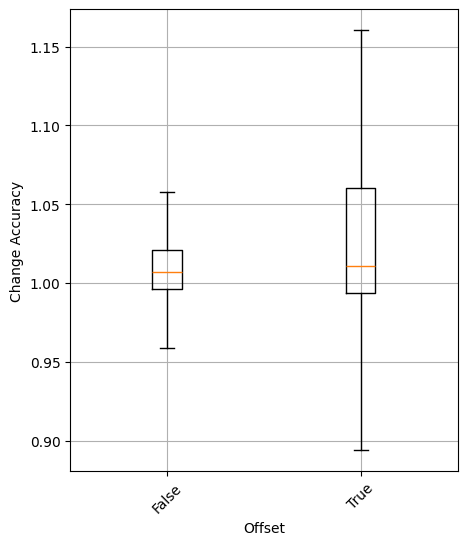
\includegraphics[width=0.95\textwidth]{plots/Offset_Trained_accuracy.png}
    \end{subfigure}
    \begin{subfigure}{0.5\textwidth}
        \centering
        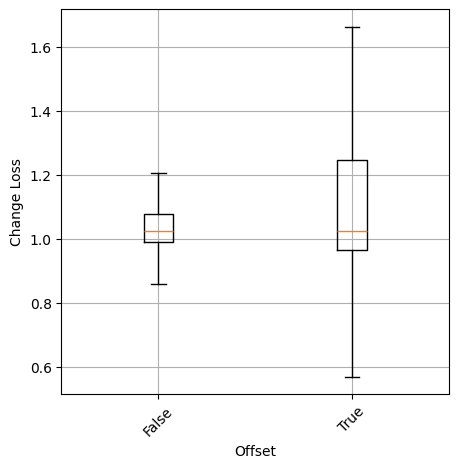
\includegraphics[width=0.95\textwidth]{plots/Offset_Trained_loss.png}
    \end{subfigure}
    \caption{Loss and accuracy, with training, with offsets or not}
    \label{fig:offset-training}
\end{figure}
\begin{figure}
    \begin{subfigure}{0.5\textwidth}
        \centering
        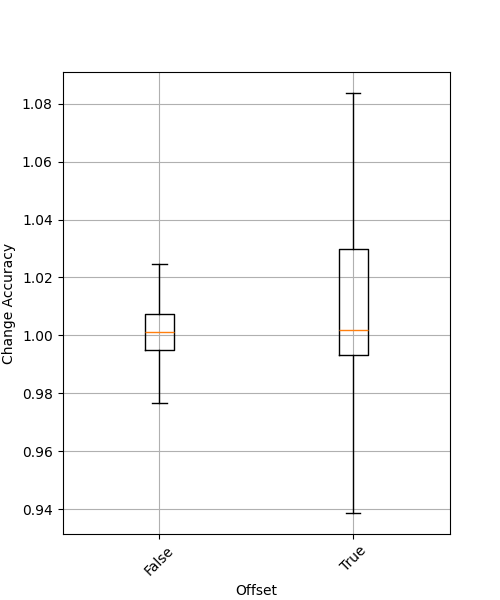
\includegraphics[width=0.95\textwidth]{plots/Offset_NotTrained_accuracy.png}
    \end{subfigure}
    \begin{subfigure}{0.5\textwidth}
        \centering
        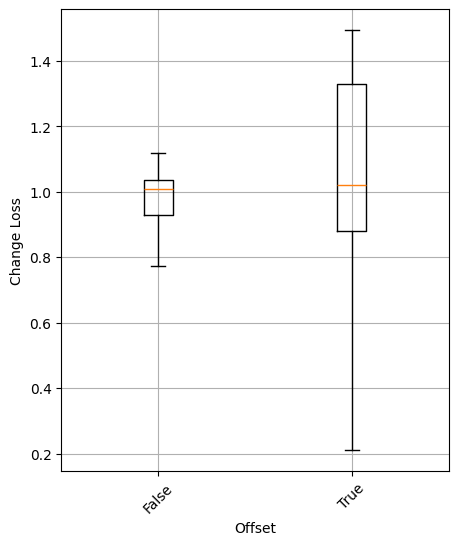
\includegraphics[width=0.95\textwidth]{plots/Offset_NotTrained_loss.png}
    \end{subfigure}
    \caption{Loss and accuracy, without training, with offsets or not}
    \label{fig:offset-notraining}
\end{figure}
\subsection{Break Conditions and Algorithm Performance}\label{subsec:break-conditions-and-algorithm-performance}
\begin{figure}
    \begin{subfigure}{0.5\textwidth}
        \centering
        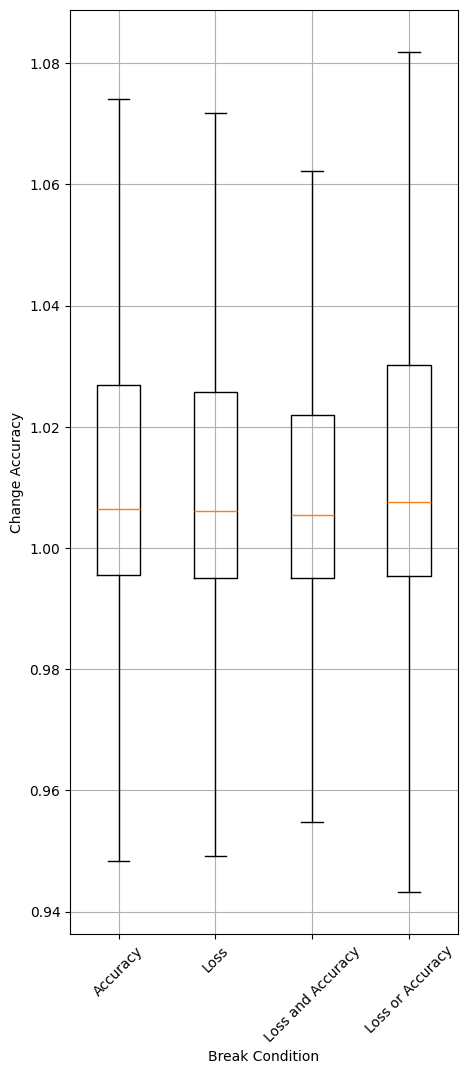
\includegraphics[width=0.95\textwidth]{plots/BreakCondition_Trained_accuracy.png}
    \end{subfigure}
    \begin{subfigure}{0.5\textwidth}
        \centering
        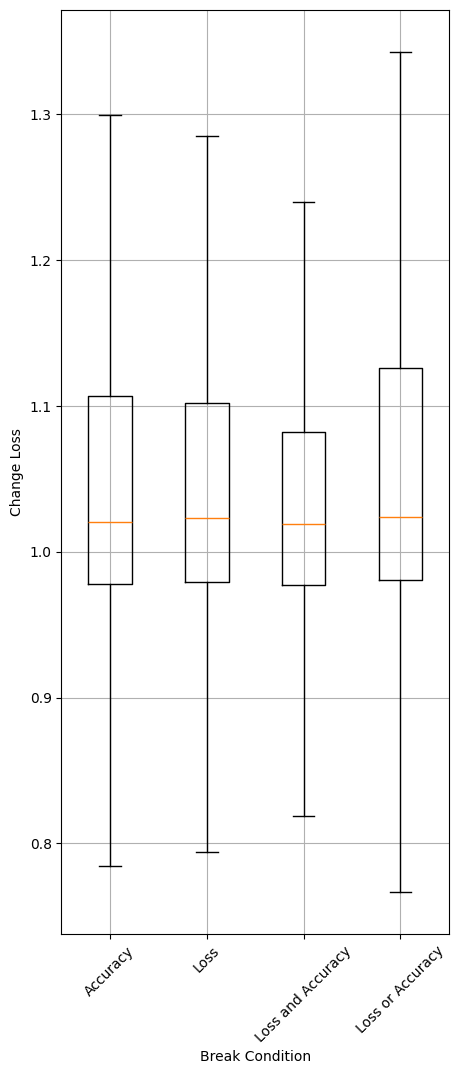
\includegraphics[width=0.95\textwidth]{plots/BreakCondition_Trained_loss.png}
    \end{subfigure}
    \caption{Loss and accuracy, with training, with different break conditions}
    \label{fig:break-conditions-training}
\end{figure}
\begin{figure}
    \begin{subfigure}{0.5\textwidth}
        \centering
        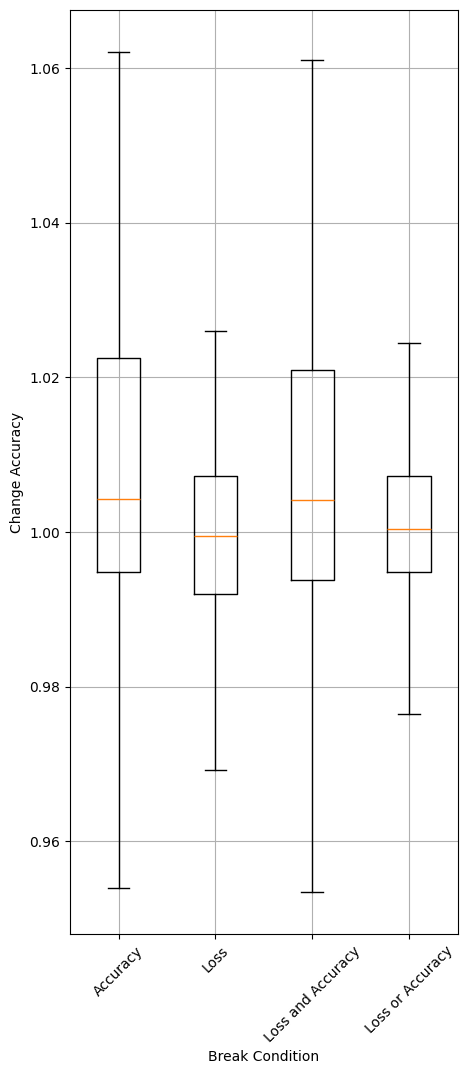
\includegraphics[width=0.95\textwidth]{plots/BreakCondition_NotTrained_accuracy.png}
    \end{subfigure}
    \begin{subfigure}{0.5\textwidth}
        \centering
        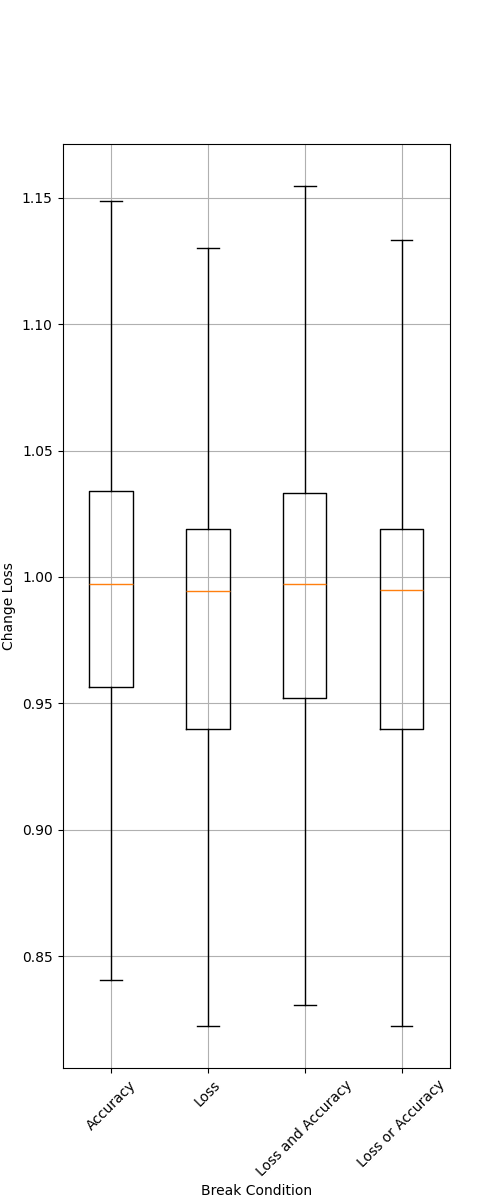
\includegraphics[width=0.95\textwidth]{plots/BreakCondition_NotTrained_loss.png}
    \end{subfigure}
    \caption{Loss and accuracy, without training, with different break conditions}
    \label{fig:break-conditions-notraining}
\end{figure}
\subsection{Contributions of Different Mutation Functions}\label{subsec:contributions-of-different-mutation-functions}
\begin{figure}
    \begin{subfigure}{0.5\textwidth}
        \centering
        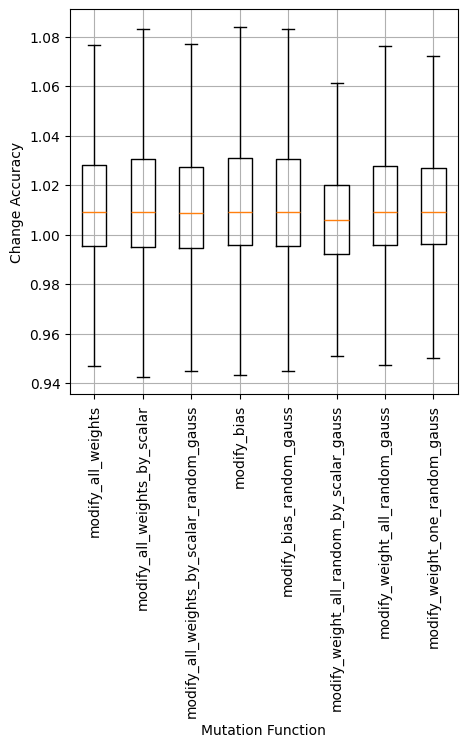
\includegraphics[width=0.95\textwidth]{plots/Mutatation_Trained_accuracy.png}
    \end{subfigure}
    \begin{subfigure}{0.5\textwidth}
        \centering
        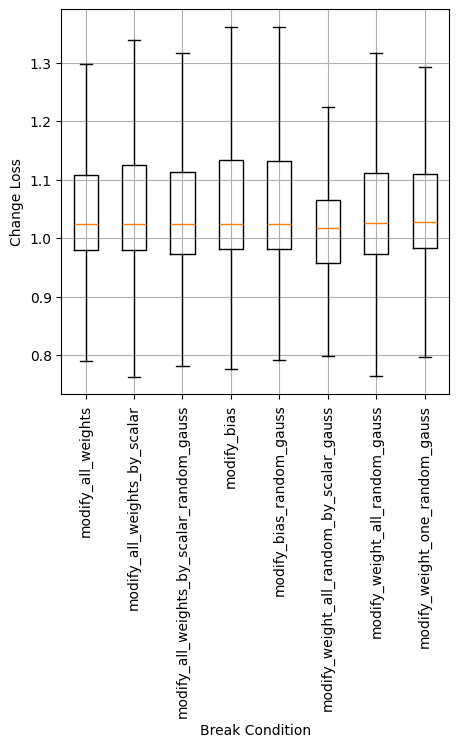
\includegraphics[width=0.95\textwidth]{plots/Mutatation_Trained_loss.png}
    \end{subfigure}
    \caption{Loss and accuracy, with training, with different mutation functions}
    \label{fig:mutation-functions-training}
\end{figure}
\begin{figure}
    \begin{subfigure}{0.5\textwidth}
        \centering
        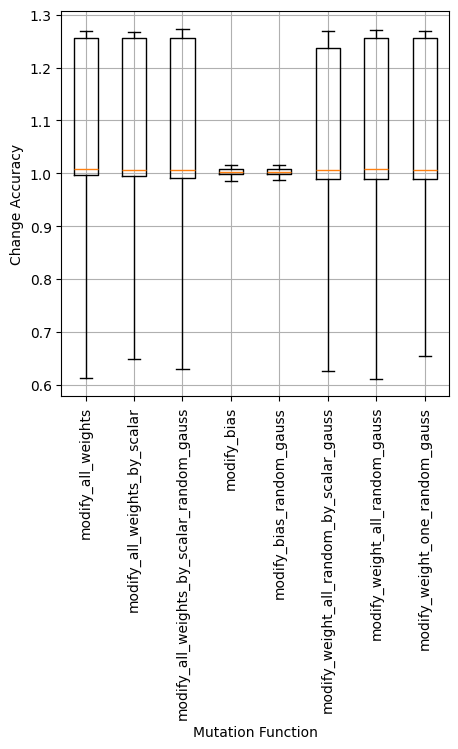
\includegraphics[width=0.95\textwidth]{plots/Mutatation_NotTrained_accuracy.png}
    \end{subfigure}
    \begin{subfigure}{0.5\textwidth}
        \centering
        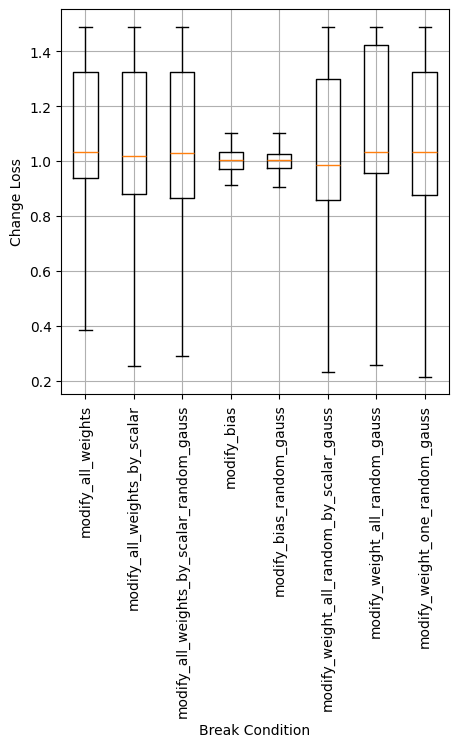
\includegraphics[width=0.95\textwidth]{plots/Mutatation_NotTrained_loss.png}
    \end{subfigure}
    \caption{Loss and accuracy, without training, with different mutation functions}
    \label{fig:mutation-functions-notraining}
\end{figure}

\chapter{Conclusion and Future Work}\label{ch:conclusion}
In the previous chapters, we introduced a new method for repairing Deep Neural Networks and Convolutional Neural Networks.
This method uses a spectrum-based fault localization combined with network mutations to increase network accuracy and decrease network loss.
First, we analyse the network to identify any faults.
We then use these findings to apply our mutation function.
If desired, we can train the network for an additional epoch.
Finally, we evaluate the network again.
If its performance has declined, we revert to the previous network.
If its performance has improved, we keep the new network and repeat the process.

During the first three epochs of our approach, we observed an increase in accuracy of up to 2--5\% for the first epoch and up to 11--25\% for untrained models.
The first epoch showed a decrease of up to 10--40\%, and the third epoch showed a decrease of up to 25--40\% compared to our benchmark, for the loss.
However, there was no further increase in accuracy for subsequent epochs, only a decrease.

If we further trained our models, we get an increase of up to 2.5-7.5\% for the accuracy and a decrease of up to 12--35\% for the loss.
Here we also see a decrease after the third epoch, but we still stay over the baseline of one for the first 10–11 epochs.

The approach performs best on the full Fashion-MNIST dataset and also good on the half data set.
For our suspiciousness measures, which we utilize for our fault localization, tarantula seems to be the best performing measure, for the trained models, the other measures aren't working significantly better than the random choosing of neurons.
The exception is in the accuracy category for the non-trained models, the Ochiai measure.
Our Approach seems to be working best on Convolutional Neural Networks, in contrast, we only see a marginal increase for Deep Neural Networks.
For our break conditions, we see no difference in the trained conditions for the trained runs, but we see one for the non-trained ones, where we see the worst performance which depends more on the loss, this holds even true for the loss.
Important is also the use of an Offset for both loss and accuracy.
Another factor that can be mitigated is the use of the different mutation functions, where we see that the mutation functions aren't leading to significantly different results, with the exception that the weight mutation function are leading to better results than the bias targeting mutation functions.

In future research, it would be beneficial to investigate several aspects.
Firstly, it is essential to evaluate the performance of the approach on larger models and more domain specific models and different datasets.
This will help to determine a threshold beyond which further modification of the neural network is impossible.
For instance, this threshold could be defined as a ratio between the model's modifiable parameters and the modified parameters.
Another thing that could be investigated in this instance is the choosing of multiple neurons at a time for the modification.

Due to time constraints, we decided to use the static spectrum matrix for fault localization instead of investigating other critical options.
A faster approach for generating the matrix should be considered.
This would lead to the possibility to change a neuron, until another more suspicious neuron arises.

One element which we also introduced due to the time constraints of this thesis is the regression for the loss and accuracy offset, to get a faster release of the break condition, hence getting runs with fewer epochs.
So the behaviour without the offset would be interesting.

Another possible area of investigation would be the suspiciousness measures, one point would be the usage of suspiciousness measures based on genetic programming which superiority in spectrum-based fault localisation regarding software was already shown by Yoo et al. \cite{yoo_human_2017} which could increase the right choosing of the neurons.
Another endeavour worth exploring would be the dstar suspiciousness measure, which we used in combination with the star value of 3, hence the investigation of values different to 3 would be needed.

A different idea would be to use the spectrum-based fault localization to not only identify suspicious neurons, but to aggregate the suspiciousness of a layer and then to modify these.
For example, we could change the activation function of the layer, the stride of a convolutional layer or pooling layer, the kernel/filter of a convolutional layer, or we could change the size of the pooling layer.
An approach, which should be tried is the freezing of an overly trustful layer could be frozen to focus on the training of the other layers.

Or another appropriate layer could be set as a predecessor or successor.
For example, a normalization layer, a dense layer or a dropout layer as a predecessor or a regularization layer as a successor.
Another idea would be the encapsulation of the layer in a residual block.
At last, we could add an attention layer on either side of the suspicious layer.

Another useful feature would be the automatically choosing of an appropriate fix when a condition is met in the suspicious neuron, like an exploding or vanishing gradient for example.
Finally, we could modify the activation function of the specified neuron using a custom layer that applies the desired activation function to each neuron, to address things like dying ReLU.

At last, we would find it beneficial to investigate some different methods for the offset in the Algorithm, to get a more precise release of the break condition.
\appendix
\chapter{Source Code}\label{ch:source-code}
\lstinputlisting[language=Python, linerange={6-40}, caption={Testing Network, for correct and incorrect classifications}, label={lst:test_model}]{source_analysis/test_network.py}
\lstinputlisting[language=Python, linerange={43-54}, caption={Testing if layer is trainable}, label={lst:test_layer_trainable}]{source_analysis/test_network.py}
\lstinputlisting[language=Python, linerange={6-57}, caption={Similarity Coefficients and Ranking}, label={lst:analysis_function}]{source_analysis/analysis.py}
\lstinputlisting[language=Python, linerange={19-81,90-123,154-195}, caption={All Saving and loading data functions}, label={lst:saving_full}]{source_analysis/utilities.py}
\lstinputlisting[language=Python, linerange={9-58}, caption={Full Modification Algorithm}, label={lst:mutation_full}]{source_mutation/__init__.py}
\lstinputlisting[language=Python, linerange={6-90}, caption={Network Testing Functions}, label={lst:full_nn_testing}]{source_analysis/test_network.py}
\backmatter
\printbibliography
\end{document}
